\documentclass[12pt,a4paper]{article}

\usepackage[a4paper,width=160mm,top=25mm,bottom=25mm]{geometry}

\usepackage{fancyhdr}
\pagestyle{fancy}
\fancyhf{}
\fancyhead[EL]{\nouppercase\leftmark}
\fancyhead[OR]{\nouppercase\rightmark}
\fancyhead[ER,OL]{\thepage}

\usepackage{url}
\usepackage[hidelinks]{hyperref}

\renewcommand{\linethickness}{0.05em}
\usepackage[brazil]{babel}   
\usepackage{titlesec}
\newcommand{\sectionbreak}{\clearpage}


\title{Processando a Informação: um livro prático de programação independente de linguagem 
\\\large\vspace{2cm}
Rogério Perino de Oliveira Neves 
\\\vspace{5mm}
Francisco de Assis Zampirolli
\\\large\vspace{2cm}
EDUFABC
\\ \url{editora.ufabc.edu.br}
\\\Huge\vspace{3cm}
Notas de Aulas inspiradas no livro
\\\Large\vspace{1cm}
Utilizando a(s) Linguagem(ns) de Programação: 
\\\Huge\vspace{1cm}
C
\\\large\vspace{1cm}
Exemplos adaptados para Correção Automática no Moodle+VPL
\vspace{2cm}}
\author{Francisco de Assis Zampirolli\vspace{1cm}}


    \usepackage[breakable]{tcolorbox}
    \usepackage{parskip} % Stop auto-indenting (to mimic markdown behaviour)
    

    % Basic figure setup, for now with no caption control since it's done
    % automatically by Pandoc (which extracts ![](path) syntax from Markdown).
    \usepackage{graphicx}
    % Maintain compatibility with old templates. Remove in nbconvert 6.0
    \let\Oldincludegraphics\includegraphics
    % Ensure that by default, figures have no caption (until we provide a
    % proper Figure object with a Caption API and a way to capture that
    % in the conversion process - todo).
    \usepackage{caption}
    \DeclareCaptionFormat{nocaption}{}
    \captionsetup{format=nocaption,aboveskip=0pt,belowskip=0pt}

    \usepackage{float}
    \floatplacement{figure}{H} % forces figures to be placed at the correct location
    \usepackage{xcolor} % Allow colors to be defined
    \usepackage{enumerate} % Needed for markdown enumerations to work
    \usepackage{geometry} % Used to adjust the document margins
    \usepackage{amsmath} % Equations
    \usepackage{amssymb} % Equations
    \usepackage{textcomp} % defines textquotesingle
    % Hack from http://tex.stackexchange.com/a/47451/13684:
    \AtBeginDocument{%
        \def\PYZsq{\textquotesingle}% Upright quotes in Pygmentized code
    }
    \usepackage{upquote} % Upright quotes for verbatim code
    \usepackage{eurosym} % defines \euro

    \usepackage{iftex}
    \ifPDFTeX
        \usepackage[T1]{fontenc}
        \IfFileExists{alphabeta.sty}{
              \usepackage{alphabeta}
          }{
              \usepackage[mathletters]{ucs}
              \usepackage[utf8x]{inputenc}
          }
    \else
        \usepackage{fontspec}
        \usepackage{unicode-math}
    \fi

    \usepackage{fancyvrb} % verbatim replacement that allows latex
    \usepackage{grffile} % extends the file name processing of package graphics
                         % to support a larger range
    \makeatletter % fix for old versions of grffile with XeLaTeX
    \@ifpackagelater{grffile}{2019/11/01}
    {
      % Do nothing on new versions
    }
    {
      \def\Gread@@xetex#1{%
        \IfFileExists{"\Gin@base".bb}%
        {\Gread@eps{\Gin@base.bb}}%
        {\Gread@@xetex@aux#1}%
      }
    }
    \makeatother
    \usepackage[Export]{adjustbox} % Used to constrain images to a maximum size
    \adjustboxset{max size={0.9\linewidth}{0.9\paperheight}}

    % The hyperref package gives us a pdf with properly built
    % internal navigation ('pdf bookmarks' for the table of contents,
    % internal cross-reference links, web links for URLs, etc.)
    \usepackage{hyperref}
    % The default LaTeX title has an obnoxious amount of whitespace. By default,
    % titling removes some of it. It also provides customization options.
    \usepackage{titling}
    \usepackage{longtable} % longtable support required by pandoc >1.10
    \usepackage{booktabs}  % table support for pandoc > 1.12.2
    \usepackage{array}     % table support for pandoc >= 2.11.3
    \usepackage{calc}      % table minipage width calculation for pandoc >= 2.11.1
    \usepackage[inline]{enumitem} % IRkernel/repr support (it uses the enumerate* environment)
    \usepackage[normalem]{ulem} % ulem is needed to support strikethroughs (\sout)
                                % normalem makes italics be italics, not underlines
    \usepackage{mathrsfs}
    

    
    % Colors for the hyperref package
    \definecolor{urlcolor}{rgb}{0,.145,.698}
    \definecolor{linkcolor}{rgb}{.71,0.21,0.01}
    \definecolor{citecolor}{rgb}{.12,.54,.11}

    % ANSI colors
    \definecolor{ansi-black}{HTML}{3E424D}
    \definecolor{ansi-black-intense}{HTML}{282C36}
    \definecolor{ansi-red}{HTML}{E75C58}
    \definecolor{ansi-red-intense}{HTML}{B22B31}
    \definecolor{ansi-green}{HTML}{00A250}
    \definecolor{ansi-green-intense}{HTML}{007427}
    \definecolor{ansi-yellow}{HTML}{DDB62B}
    \definecolor{ansi-yellow-intense}{HTML}{B27D12}
    \definecolor{ansi-blue}{HTML}{208FFB}
    \definecolor{ansi-blue-intense}{HTML}{0065CA}
    \definecolor{ansi-magenta}{HTML}{D160C4}
    \definecolor{ansi-magenta-intense}{HTML}{A03196}
    \definecolor{ansi-cyan}{HTML}{60C6C8}
    \definecolor{ansi-cyan-intense}{HTML}{258F8F}
    \definecolor{ansi-white}{HTML}{C5C1B4}
    \definecolor{ansi-white-intense}{HTML}{A1A6B2}
    \definecolor{ansi-default-inverse-fg}{HTML}{FFFFFF}
    \definecolor{ansi-default-inverse-bg}{HTML}{000000}

    % common color for the border for error outputs.
    \definecolor{outerrorbackground}{HTML}{FFDFDF}

    % commands and environments needed by pandoc snippets
    % extracted from the output of `pandoc -s`
    \providecommand{\tightlist}{%
      \setlength{\itemsep}{0pt}\setlength{\parskip}{0pt}}
    \DefineVerbatimEnvironment{Highlighting}{Verbatim}{commandchars=\\\{\}}
    % Add ',fontsize=\small' for more characters per line
    \newenvironment{Shaded}{}{}
    \newcommand{\KeywordTok}[1]{\textcolor[rgb]{0.00,0.44,0.13}{\textbf{{#1}}}}
    \newcommand{\DataTypeTok}[1]{\textcolor[rgb]{0.56,0.13,0.00}{{#1}}}
    \newcommand{\DecValTok}[1]{\textcolor[rgb]{0.25,0.63,0.44}{{#1}}}
    \newcommand{\BaseNTok}[1]{\textcolor[rgb]{0.25,0.63,0.44}{{#1}}}
    \newcommand{\FloatTok}[1]{\textcolor[rgb]{0.25,0.63,0.44}{{#1}}}
    \newcommand{\CharTok}[1]{\textcolor[rgb]{0.25,0.44,0.63}{{#1}}}
    \newcommand{\StringTok}[1]{\textcolor[rgb]{0.25,0.44,0.63}{{#1}}}
    \newcommand{\CommentTok}[1]{\textcolor[rgb]{0.38,0.63,0.69}{\textit{{#1}}}}
    \newcommand{\OtherTok}[1]{\textcolor[rgb]{0.00,0.44,0.13}{{#1}}}
    \newcommand{\AlertTok}[1]{\textcolor[rgb]{1.00,0.00,0.00}{\textbf{{#1}}}}
    \newcommand{\FunctionTok}[1]{\textcolor[rgb]{0.02,0.16,0.49}{{#1}}}
    \newcommand{\RegionMarkerTok}[1]{{#1}}
    \newcommand{\ErrorTok}[1]{\textcolor[rgb]{1.00,0.00,0.00}{\textbf{{#1}}}}
    \newcommand{\NormalTok}[1]{{#1}}

    % Additional commands for more recent versions of Pandoc
    \newcommand{\ConstantTok}[1]{\textcolor[rgb]{0.53,0.00,0.00}{{#1}}}
    \newcommand{\SpecialCharTok}[1]{\textcolor[rgb]{0.25,0.44,0.63}{{#1}}}
    \newcommand{\VerbatimStringTok}[1]{\textcolor[rgb]{0.25,0.44,0.63}{{#1}}}
    \newcommand{\SpecialStringTok}[1]{\textcolor[rgb]{0.73,0.40,0.53}{{#1}}}
    \newcommand{\ImportTok}[1]{{#1}}
    \newcommand{\DocumentationTok}[1]{\textcolor[rgb]{0.73,0.13,0.13}{\textit{{#1}}}}
    \newcommand{\AnnotationTok}[1]{\textcolor[rgb]{0.38,0.63,0.69}{\textbf{\textit{{#1}}}}}
    \newcommand{\CommentVarTok}[1]{\textcolor[rgb]{0.38,0.63,0.69}{\textbf{\textit{{#1}}}}}
    \newcommand{\VariableTok}[1]{\textcolor[rgb]{0.10,0.09,0.49}{{#1}}}
    \newcommand{\ControlFlowTok}[1]{\textcolor[rgb]{0.00,0.44,0.13}{\textbf{{#1}}}}
    \newcommand{\OperatorTok}[1]{\textcolor[rgb]{0.40,0.40,0.40}{{#1}}}
    \newcommand{\BuiltInTok}[1]{{#1}}
    \newcommand{\ExtensionTok}[1]{{#1}}
    \newcommand{\PreprocessorTok}[1]{\textcolor[rgb]{0.74,0.48,0.00}{{#1}}}
    \newcommand{\AttributeTok}[1]{\textcolor[rgb]{0.49,0.56,0.16}{{#1}}}
    \newcommand{\InformationTok}[1]{\textcolor[rgb]{0.38,0.63,0.69}{\textbf{\textit{{#1}}}}}
    \newcommand{\WarningTok}[1]{\textcolor[rgb]{0.38,0.63,0.69}{\textbf{\textit{{#1}}}}}


    % Define a nice break command that doesn't care if a line doesn't already
    % exist.
    \def\br{\hspace*{\fill} \\* }
    % Math Jax compatibility definitions
    \def\gt{>}
    \def\lt{<}
    \let\Oldtex\TeX
    \let\Oldlatex\LaTeX
    \renewcommand{\TeX}{\textrm{\Oldtex}}
    \renewcommand{\LaTeX}{\textrm{\Oldlatex}}
    % Document parameters
    % Document title
    %\title{cap5.part1.c}
    
    
    
    
    
% Pygments definitions
\makeatletter
\def\PY@reset{\let\PY@it=\relax \let\PY@bf=\relax%
    \let\PY@ul=\relax \let\PY@tc=\relax%
    \let\PY@bc=\relax \let\PY@ff=\relax}
\def\PY@tok#1{\csname PY@tok@#1\endcsname}
\def\PY@toks#1+{\ifx\relax#1\empty\else%
    \PY@tok{#1}\expandafter\PY@toks\fi}
\def\PY@do#1{\PY@bc{\PY@tc{\PY@ul{%
    \PY@it{\PY@bf{\PY@ff{#1}}}}}}}
\def\PY#1#2{\PY@reset\PY@toks#1+\relax+\PY@do{#2}}

\@namedef{PY@tok@w}{\def\PY@tc##1{\textcolor[rgb]{0.73,0.73,0.73}{##1}}}
\@namedef{PY@tok@c}{\let\PY@it=\textit\def\PY@tc##1{\textcolor[rgb]{0.24,0.48,0.48}{##1}}}
\@namedef{PY@tok@cp}{\def\PY@tc##1{\textcolor[rgb]{0.61,0.40,0.00}{##1}}}
\@namedef{PY@tok@k}{\let\PY@bf=\textbf\def\PY@tc##1{\textcolor[rgb]{0.00,0.50,0.00}{##1}}}
\@namedef{PY@tok@kp}{\def\PY@tc##1{\textcolor[rgb]{0.00,0.50,0.00}{##1}}}
\@namedef{PY@tok@kt}{\def\PY@tc##1{\textcolor[rgb]{0.69,0.00,0.25}{##1}}}
\@namedef{PY@tok@o}{\def\PY@tc##1{\textcolor[rgb]{0.40,0.40,0.40}{##1}}}
\@namedef{PY@tok@ow}{\let\PY@bf=\textbf\def\PY@tc##1{\textcolor[rgb]{0.67,0.13,1.00}{##1}}}
\@namedef{PY@tok@nb}{\def\PY@tc##1{\textcolor[rgb]{0.00,0.50,0.00}{##1}}}
\@namedef{PY@tok@nf}{\def\PY@tc##1{\textcolor[rgb]{0.00,0.00,1.00}{##1}}}
\@namedef{PY@tok@nc}{\let\PY@bf=\textbf\def\PY@tc##1{\textcolor[rgb]{0.00,0.00,1.00}{##1}}}
\@namedef{PY@tok@nn}{\let\PY@bf=\textbf\def\PY@tc##1{\textcolor[rgb]{0.00,0.00,1.00}{##1}}}
\@namedef{PY@tok@ne}{\let\PY@bf=\textbf\def\PY@tc##1{\textcolor[rgb]{0.80,0.25,0.22}{##1}}}
\@namedef{PY@tok@nv}{\def\PY@tc##1{\textcolor[rgb]{0.10,0.09,0.49}{##1}}}
\@namedef{PY@tok@no}{\def\PY@tc##1{\textcolor[rgb]{0.53,0.00,0.00}{##1}}}
\@namedef{PY@tok@nl}{\def\PY@tc##1{\textcolor[rgb]{0.46,0.46,0.00}{##1}}}
\@namedef{PY@tok@ni}{\let\PY@bf=\textbf\def\PY@tc##1{\textcolor[rgb]{0.44,0.44,0.44}{##1}}}
\@namedef{PY@tok@na}{\def\PY@tc##1{\textcolor[rgb]{0.41,0.47,0.13}{##1}}}
\@namedef{PY@tok@nt}{\let\PY@bf=\textbf\def\PY@tc##1{\textcolor[rgb]{0.00,0.50,0.00}{##1}}}
\@namedef{PY@tok@nd}{\def\PY@tc##1{\textcolor[rgb]{0.67,0.13,1.00}{##1}}}
\@namedef{PY@tok@s}{\def\PY@tc##1{\textcolor[rgb]{0.73,0.13,0.13}{##1}}}
\@namedef{PY@tok@sd}{\let\PY@it=\textit\def\PY@tc##1{\textcolor[rgb]{0.73,0.13,0.13}{##1}}}
\@namedef{PY@tok@si}{\let\PY@bf=\textbf\def\PY@tc##1{\textcolor[rgb]{0.64,0.35,0.47}{##1}}}
\@namedef{PY@tok@se}{\let\PY@bf=\textbf\def\PY@tc##1{\textcolor[rgb]{0.67,0.36,0.12}{##1}}}
\@namedef{PY@tok@sr}{\def\PY@tc##1{\textcolor[rgb]{0.64,0.35,0.47}{##1}}}
\@namedef{PY@tok@ss}{\def\PY@tc##1{\textcolor[rgb]{0.10,0.09,0.49}{##1}}}
\@namedef{PY@tok@sx}{\def\PY@tc##1{\textcolor[rgb]{0.00,0.50,0.00}{##1}}}
\@namedef{PY@tok@m}{\def\PY@tc##1{\textcolor[rgb]{0.40,0.40,0.40}{##1}}}
\@namedef{PY@tok@gh}{\let\PY@bf=\textbf\def\PY@tc##1{\textcolor[rgb]{0.00,0.00,0.50}{##1}}}
\@namedef{PY@tok@gu}{\let\PY@bf=\textbf\def\PY@tc##1{\textcolor[rgb]{0.50,0.00,0.50}{##1}}}
\@namedef{PY@tok@gd}{\def\PY@tc##1{\textcolor[rgb]{0.63,0.00,0.00}{##1}}}
\@namedef{PY@tok@gi}{\def\PY@tc##1{\textcolor[rgb]{0.00,0.52,0.00}{##1}}}
\@namedef{PY@tok@gr}{\def\PY@tc##1{\textcolor[rgb]{0.89,0.00,0.00}{##1}}}
\@namedef{PY@tok@ge}{\let\PY@it=\textit}
\@namedef{PY@tok@gs}{\let\PY@bf=\textbf}
\@namedef{PY@tok@gp}{\let\PY@bf=\textbf\def\PY@tc##1{\textcolor[rgb]{0.00,0.00,0.50}{##1}}}
\@namedef{PY@tok@go}{\def\PY@tc##1{\textcolor[rgb]{0.44,0.44,0.44}{##1}}}
\@namedef{PY@tok@gt}{\def\PY@tc##1{\textcolor[rgb]{0.00,0.27,0.87}{##1}}}
\@namedef{PY@tok@err}{\def\PY@bc##1{{\setlength{\fboxsep}{\string -\fboxrule}\fcolorbox[rgb]{1.00,0.00,0.00}{1,1,1}{\strut ##1}}}}
\@namedef{PY@tok@kc}{\let\PY@bf=\textbf\def\PY@tc##1{\textcolor[rgb]{0.00,0.50,0.00}{##1}}}
\@namedef{PY@tok@kd}{\let\PY@bf=\textbf\def\PY@tc##1{\textcolor[rgb]{0.00,0.50,0.00}{##1}}}
\@namedef{PY@tok@kn}{\let\PY@bf=\textbf\def\PY@tc##1{\textcolor[rgb]{0.00,0.50,0.00}{##1}}}
\@namedef{PY@tok@kr}{\let\PY@bf=\textbf\def\PY@tc##1{\textcolor[rgb]{0.00,0.50,0.00}{##1}}}
\@namedef{PY@tok@bp}{\def\PY@tc##1{\textcolor[rgb]{0.00,0.50,0.00}{##1}}}
\@namedef{PY@tok@fm}{\def\PY@tc##1{\textcolor[rgb]{0.00,0.00,1.00}{##1}}}
\@namedef{PY@tok@vc}{\def\PY@tc##1{\textcolor[rgb]{0.10,0.09,0.49}{##1}}}
\@namedef{PY@tok@vg}{\def\PY@tc##1{\textcolor[rgb]{0.10,0.09,0.49}{##1}}}
\@namedef{PY@tok@vi}{\def\PY@tc##1{\textcolor[rgb]{0.10,0.09,0.49}{##1}}}
\@namedef{PY@tok@vm}{\def\PY@tc##1{\textcolor[rgb]{0.10,0.09,0.49}{##1}}}
\@namedef{PY@tok@sa}{\def\PY@tc##1{\textcolor[rgb]{0.73,0.13,0.13}{##1}}}
\@namedef{PY@tok@sb}{\def\PY@tc##1{\textcolor[rgb]{0.73,0.13,0.13}{##1}}}
\@namedef{PY@tok@sc}{\def\PY@tc##1{\textcolor[rgb]{0.73,0.13,0.13}{##1}}}
\@namedef{PY@tok@dl}{\def\PY@tc##1{\textcolor[rgb]{0.73,0.13,0.13}{##1}}}
\@namedef{PY@tok@s2}{\def\PY@tc##1{\textcolor[rgb]{0.73,0.13,0.13}{##1}}}
\@namedef{PY@tok@sh}{\def\PY@tc##1{\textcolor[rgb]{0.73,0.13,0.13}{##1}}}
\@namedef{PY@tok@s1}{\def\PY@tc##1{\textcolor[rgb]{0.73,0.13,0.13}{##1}}}
\@namedef{PY@tok@mb}{\def\PY@tc##1{\textcolor[rgb]{0.40,0.40,0.40}{##1}}}
\@namedef{PY@tok@mf}{\def\PY@tc##1{\textcolor[rgb]{0.40,0.40,0.40}{##1}}}
\@namedef{PY@tok@mh}{\def\PY@tc##1{\textcolor[rgb]{0.40,0.40,0.40}{##1}}}
\@namedef{PY@tok@mi}{\def\PY@tc##1{\textcolor[rgb]{0.40,0.40,0.40}{##1}}}
\@namedef{PY@tok@il}{\def\PY@tc##1{\textcolor[rgb]{0.40,0.40,0.40}{##1}}}
\@namedef{PY@tok@mo}{\def\PY@tc##1{\textcolor[rgb]{0.40,0.40,0.40}{##1}}}
\@namedef{PY@tok@ch}{\let\PY@it=\textit\def\PY@tc##1{\textcolor[rgb]{0.24,0.48,0.48}{##1}}}
\@namedef{PY@tok@cm}{\let\PY@it=\textit\def\PY@tc##1{\textcolor[rgb]{0.24,0.48,0.48}{##1}}}
\@namedef{PY@tok@cpf}{\let\PY@it=\textit\def\PY@tc##1{\textcolor[rgb]{0.24,0.48,0.48}{##1}}}
\@namedef{PY@tok@c1}{\let\PY@it=\textit\def\PY@tc##1{\textcolor[rgb]{0.24,0.48,0.48}{##1}}}
\@namedef{PY@tok@cs}{\let\PY@it=\textit\def\PY@tc##1{\textcolor[rgb]{0.24,0.48,0.48}{##1}}}

\def\PYZbs{\char`\\}
\def\PYZus{\char`\_}
\def\PYZob{\char`\{}
\def\PYZcb{\char`\}}
\def\PYZca{\char`\^}
\def\PYZam{\char`\&}
\def\PYZlt{\char`\<}
\def\PYZgt{\char`\>}
\def\PYZsh{\char`\#}
\def\PYZpc{\char`\%}
\def\PYZdl{\char`\$}
\def\PYZhy{\char`\-}
\def\PYZsq{\char`\'}
\def\PYZdq{\char`\"}
\def\PYZti{\char`\~}
% for compatibility with earlier versions
\def\PYZat{@}
\def\PYZlb{[}
\def\PYZrb{]}
\makeatother


    % For linebreaks inside Verbatim environment from package fancyvrb.
    \makeatletter
        \newbox\Wrappedcontinuationbox
        \newbox\Wrappedvisiblespacebox
        \newcommand*\Wrappedvisiblespace {\textcolor{red}{\textvisiblespace}}
        \newcommand*\Wrappedcontinuationsymbol {\textcolor{red}{\llap{\tiny$\m@th\hookrightarrow$}}}
        \newcommand*\Wrappedcontinuationindent {3ex }
        \newcommand*\Wrappedafterbreak {\kern\Wrappedcontinuationindent\copy\Wrappedcontinuationbox}
        % Take advantage of the already applied Pygments mark-up to insert
        % potential linebreaks for TeX processing.
        %        {, <, #, %, $, ' and ": go to next line.
        %        _, }, ^, &, >, - and ~: stay at end of broken line.
        % Use of \textquotesingle for straight quote.
        \newcommand*\Wrappedbreaksatspecials {%
            \def\PYGZus{\discretionary{\char`\_}{\Wrappedafterbreak}{\char`\_}}%
            \def\PYGZob{\discretionary{}{\Wrappedafterbreak\char`\{}{\char`\{}}%
            \def\PYGZcb{\discretionary{\char`\}}{\Wrappedafterbreak}{\char`\}}}%
            \def\PYGZca{\discretionary{\char`\^}{\Wrappedafterbreak}{\char`\^}}%
            \def\PYGZam{\discretionary{\char`\&}{\Wrappedafterbreak}{\char`\&}}%
            \def\PYGZlt{\discretionary{}{\Wrappedafterbreak\char`\<}{\char`\<}}%
            \def\PYGZgt{\discretionary{\char`\>}{\Wrappedafterbreak}{\char`\>}}%
            \def\PYGZsh{\discretionary{}{\Wrappedafterbreak\char`\#}{\char`\#}}%
            \def\PYGZpc{\discretionary{}{\Wrappedafterbreak\char`\%}{\char`\%}}%
            \def\PYGZdl{\discretionary{}{\Wrappedafterbreak\char`\$}{\char`\$}}%
            \def\PYGZhy{\discretionary{\char`\-}{\Wrappedafterbreak}{\char`\-}}%
            \def\PYGZsq{\discretionary{}{\Wrappedafterbreak\textquotesingle}{\textquotesingle}}%
            \def\PYGZdq{\discretionary{}{\Wrappedafterbreak\char`\"}{\char`\"}}%
            \def\PYGZti{\discretionary{\char`\~}{\Wrappedafterbreak}{\char`\~}}%
        }
        % Some characters . , ; ? ! / are not pygmentized.
        % This macro makes them "active" and they will insert potential linebreaks
        \newcommand*\Wrappedbreaksatpunct {%
            \lccode`\~`\.\lowercase{\def~}{\discretionary{\hbox{\char`\.}}{\Wrappedafterbreak}{\hbox{\char`\.}}}%
            \lccode`\~`\,\lowercase{\def~}{\discretionary{\hbox{\char`\,}}{\Wrappedafterbreak}{\hbox{\char`\,}}}%
            \lccode`\~`\;\lowercase{\def~}{\discretionary{\hbox{\char`\;}}{\Wrappedafterbreak}{\hbox{\char`\;}}}%
            \lccode`\~`\:\lowercase{\def~}{\discretionary{\hbox{\char`\:}}{\Wrappedafterbreak}{\hbox{\char`\:}}}%
            \lccode`\~`\?\lowercase{\def~}{\discretionary{\hbox{\char`\?}}{\Wrappedafterbreak}{\hbox{\char`\?}}}%
            \lccode`\~`\!\lowercase{\def~}{\discretionary{\hbox{\char`\!}}{\Wrappedafterbreak}{\hbox{\char`\!}}}%
            \lccode`\~`\/\lowercase{\def~}{\discretionary{\hbox{\char`\/}}{\Wrappedafterbreak}{\hbox{\char`\/}}}%
            \catcode`\.\active
            \catcode`\,\active
            \catcode`\;\active
            \catcode`\:\active
            \catcode`\?\active
            \catcode`\!\active
            \catcode`\/\active
            \lccode`\~`\~
        }
    \makeatother

    \let\OriginalVerbatim=\Verbatim
    \makeatletter
    \renewcommand{\Verbatim}[1][1]{%
        %\parskip\z@skip
        \sbox\Wrappedcontinuationbox {\Wrappedcontinuationsymbol}%
        \sbox\Wrappedvisiblespacebox {\FV@SetupFont\Wrappedvisiblespace}%
        \def\FancyVerbFormatLine ##1{\hsize\linewidth
            \vtop{\raggedright\hyphenpenalty\z@\exhyphenpenalty\z@
                \doublehyphendemerits\z@\finalhyphendemerits\z@
                \strut ##1\strut}%
        }%
        % If the linebreak is at a space, the latter will be displayed as visible
        % space at end of first line, and a continuation symbol starts next line.
        % Stretch/shrink are however usually zero for typewriter font.
        \def\FV@Space {%
            \nobreak\hskip\z@ plus\fontdimen3\font minus\fontdimen4\font
            \discretionary{\copy\Wrappedvisiblespacebox}{\Wrappedafterbreak}
            {\kern\fontdimen2\font}%
        }%

        % Allow breaks at special characters using \PYG... macros.
        \Wrappedbreaksatspecials
        % Breaks at punctuation characters . , ; ? ! and / need catcode=\active
        \OriginalVerbatim[#1,codes*=\Wrappedbreaksatpunct]%
    }
    \makeatother

    % Exact colors from NB
    \definecolor{incolor}{HTML}{303F9F}
    \definecolor{outcolor}{HTML}{D84315}
    \definecolor{cellborder}{HTML}{CFCFCF}
    \definecolor{cellbackground}{HTML}{F7F7F7}

    % prompt
    \makeatletter
    \newcommand{\boxspacing}{\kern\kvtcb@left@rule\kern\kvtcb@boxsep}
    \makeatother
    \newcommand{\prompt}[4]{
        {\ttfamily\llap{{\color{#2}[#3]:\hspace{3pt}#4}}\vspace{-\baselineskip}}
    }
    

    
    % Prevent overflowing lines due to hard-to-break entities
    \sloppy
    % Setup hyperref package
    \hypersetup{
      breaklinks=true,  % so long urls are correctly broken across lines
      colorlinks=true,
      urlcolor=urlcolor,
      linkcolor=linkcolor,
      citecolor=citecolor,
      }
    % Slightly bigger margins than the latex defaults
    
    \geometry{verbose,tmargin=1in,bmargin=1in,lmargin=1in,rmargin=1in}
    
    

\begin{document}
    
    
\clearpage\maketitle
\thispagestyle{empty}
\tableofcontents

    
    

    
    \hypertarget{processando-a-informauxe7uxe3o-cap.-5-vetores}{%
\section{Processando a Informação: Cap. 5:
Vetores}\label{processando-a-informauxe7uxe3o-cap.-5-vetores}}

    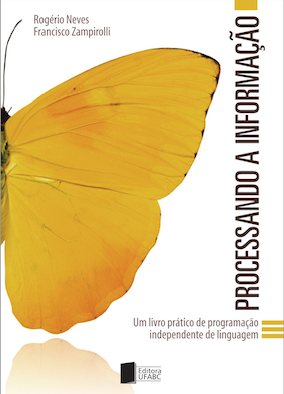
\includegraphics{"figs/Capa_Processando_Informacao.jpg"}

Este caderno (Notebook) é parte complementar \emph{online} do livro
\textbf{\href{https://editora.ufabc.edu.br/matematica-e-ciencias-da-computacao/58-processando-a-informacao}{Processando
a Informação}: um livro prático de programação independente de
linguagem}, que deve ser consultado no caso de dúvidas sobre os temas
apresentados.

\begin{quote}
Este conteúdo pode ser copiado e alterado livremente e foi inspirado
nesse livro.
\end{quote}

    \hypertarget{sumuxe1rio}{%
\subsection{Sumário}\label{sumuxe1rio}}

\begin{itemize}
\tightlist
\item
  Revisão do capítulo anterior
\item
  Introdução
\item
  Trabalhando com vetores
\item
  Acessando elementos de um vetor
\item
  Formas de percorrer um vetor
\item
  Modularização e vetores
\item
  Revisão deste capítulo
\item
  Exercícios
\end{itemize}

    \hypertarget{revisuxe3o-do-capuxedtulo-anterior-estruturas-de-repetiuxe7uxe3o---lauxe7os}{%
\subsection{Revisão do capítulo anterior (Estruturas de Repetição -
Laços)}\label{revisuxe3o-do-capuxedtulo-anterior-estruturas-de-repetiuxe7uxe3o---lauxe7os}}

    \begin{itemize}
\tightlist
\item
  Estruturas de repetição (laços) devem ser utilizadas quando existem
  instruções que se repentem e podem ser de vários tipos, dependendo da
  linguagem utilizada, por exemplo:

  \begin{itemize}
  \tightlist
  \item
    \texttt{do-while} (não aceita em Python)
  \item
    \texttt{while} (a maioria)
  \item
    \texttt{for} (a maioria)
  \item
    \texttt{repeat} (R)
  \end{itemize}
\item
  O uso de laços depende da lógica a ser implementada e da linguagem
  utilizada. Mas, se tiver um número fixo de iterações, geralmente se
  usa \texttt{for}.
\item
  Validação de dados utilizando laços:

  \begin{itemize}
  \tightlist
  \item
    Incluir um laço para verificar o valor lido.
  \end{itemize}
\item
  Interrupção da execução em laços:

  \begin{itemize}
  \tightlist
  \item
    Depende da linguagem, algumas possibilidades:

    \begin{itemize}
    \tightlist
    \item
      \texttt{break} - interrompe o laço
    \item
      \texttt{continue} - não executa o final do laço
    \item
      \texttt{exit} - aborta o laço e o programa!
    \end{itemize}
  \end{itemize}
\item
  Neste capítulo iremos abordar a estrutura de \textbf{Vetor}, incluindo
  os conceitos apresentados nos capítulos anteriores.
\end{itemize}

    \hypertarget{introduuxe7uxe3o}{%
\subsection{Introdução}\label{introduuxe7uxe3o}}

    \begin{itemize}
\tightlist
\item
  Um \textbf{vetor} em programação é formado por um \textbf{conjunto de
  \(n\) variáveis de um mesmo tipo} de dado (em geral), sendo \(n\)
  obrigatoriamente maior que zero.
\item
  Essas variáveis (ou elementos) são identificadas e acessadas por um
  \textbf{nome} e um \textbf{índice}.
\item
  Na maioria das linguagens de programação, o \textbf{índice} recebe
  valores de \(0\) (\textbf{primeiro elemento}) até \(n-1\)
  (\textbf{último elemento}).\\
\item
  As variáveis de um vetor são armazenadas em posições consecutivas de
  memória.
\end{itemize}

    \hypertarget{trabalhando-com-vetores}{%
\subsection{Trabalhando com vetores}\label{trabalhando-com-vetores}}

    \begin{itemize}
\tightlist
\item
  Quando um vetor é criado, é instanciada uma variável do tipo vetor (em
  algumas linguagens de programação, sendo necessário se definir um
  nome, o tipo de dado e o tamanho do vetor).
\item
  Na linguagem C, por exemplo, a definição do tamanho de um vetor ocorre
  antes de compilar o programa.

  \begin{itemize}
  \tightlist
  \item
    Ou seja, o programador deverá informar no código a quantidade de
    memória a ser reservada para o vetor, através de um número inteiro
    positivo ou constante que o contenha, especificando o número de
    elementos do mesmo tipo que a memória reservada irá comportar.
  \item
    Neste caso, uma variável não pode ser usada.
  \end{itemize}
\item
  Já na linguagem Java, é possível alocar memória em tempo de execução
  do programa.

  \begin{itemize}
  \tightlist
  \item
    Por exemplo, é possível criar um vetor para armazenar as notas de
    uma turma de alunos, onde o número de alunos é uma variável a ser
    lida durante a execução do programa.
  \end{itemize}
\end{itemize}

    \begin{itemize}
\tightlist
\item
  Em muitas linguagens, como Java e C, o processo de criar um vetor
  ocorre em dois passos distintos:

  \begin{enumerate}
  \def\labelenumi{\arabic{enumi}.}
  \tightlist
  \item
    primeiro se cria uma variável de referência para o vetor;
  \item
    em seguida se reserva a memória para um dado número de elementos do
    mesmo tipo.
  \end{enumerate}
\item
  No exemplo da figura abaixo,

  \begin{itemize}
  \tightlist
  \item
    a criação da variável de referência de um vetor \texttt{v} define
    apenas a posição de memória em hexadecimal \texttt{0A}, onde será
    armazenado o seu primeiro elemento.

    \begin{itemize}
    \tightlist
    \item
      neste exemplo, \texttt{V{[}0{]}\ =\ -128} é o primeiro elemento do
      vetor.
    \item
      a quantidade de \texttt{bytes} por elemento vai depender to tipo
      de dado armazenado. Neste exemplo cada elemento ocupa um
      \texttt{byte}.
    \end{itemize}
  \item
    o segundo passo da criação de um vetor é reservar (ou alocar)
    memória para todos os seus elementos (dependendo da linguagem).
    \textgreater{} essa alocação de memória pode ocorrer em tempo de
    execução, como ocorre em Python!
  \end{itemize}
\end{itemize}

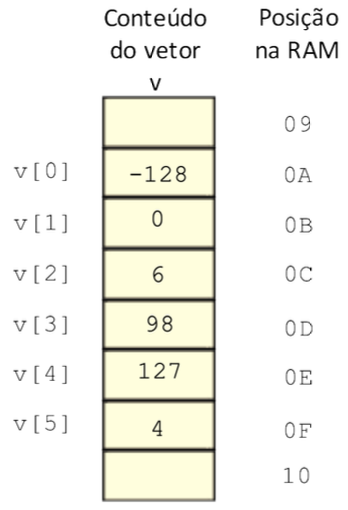
\includegraphics{"figs/image33.png"}

    \begin{figure}
\centering
\caption{image.png}
\end{figure}

    \begin{itemize}
\tightlist
\item
  Note que a variável \texttt{v} acima agora se refere a uma posição de
  memória e não a um elemento de dado.
\item
  Os elementos devem ser acessados através do índice, um por vez.
\item
  Isso pode requerer uso de laços para leitura e impressão dos seus
  elementos, dependendo da linguagem de programação utilizada.

  \begin{itemize}
  \tightlist
  \item
    O índice de vetor é sempre um número inteiro.
  \end{itemize}
\end{itemize}

    \hypertarget{exemplo-01---lerescrever-vetor}{%
\subsection{Exemplo 01 - Ler/Escrever
vetor}\label{exemplo-01---lerescrever-vetor}}

    \hypertarget{pseudocuxf3digo}{%
\paragraph{Pseudocódigo}\label{pseudocuxf3digo}}

    \begin{verbatim}
Instanciar o vetor v1 de inteiro com tamanho 5 // ou
vetor v2 = vetor de inteiros com 100 elementos // ou ainda
vetor v3 = inteiro(10)
v1 = {4,1,10,2,3} // atribuindo valores a v1
\end{verbatim}

    \textbf{Exemplo 01:} Ler uma lista com \texttt{n} alunos com \texttt{RA}
e \texttt{Nome} e escrever formatando a saída como no exemplo:

    \begin{verbatim}
LISTA DE ALUNOS
Número RA     Nome
1      2134   Maria Campos
2      346    João Silva
\end{verbatim}

    \hypertarget{casos-para-teste-moodlevpl}{%
\paragraph{Casos para Teste
Moodle+VPL}\label{casos-para-teste-moodlevpl}}

Para o professor criar uma atividade VPL no Moodle para este Exemplo 01,
basta incluir em \texttt{Casos\ para\ teste}, o seguinte texto (pode
incluir mais casos):

\begin{verbatim}
case=caso1
input=2
2345
9870
Maria Campos
João Silva
output= 
LISTA DE ALUNOS
Número RA     Nota
1      2345   Maria Campos
2      9870   João Silva
\end{verbatim}

    \begin{tcolorbox}[breakable, size=fbox, boxrule=1pt, pad at break*=1mm,colback=cellbackground, colframe=cellborder]
\prompt{In}{incolor}{ }{\boxspacing}
\begin{Verbatim}[commandchars=\\\{\}]
\PY{o}{\PYZpc{}\PYZpc{}writefile} cap5ex01.c
\PY{c+c1}{\PYZsh{}include \PYZlt{}stdio.h\PYZgt{}}

\PY{n+nb}{int} \PY{n}{main}\PY{p}{(}\PY{n}{void}\PY{p}{)} \PY{p}{\PYZob{}}

  \PY{o}{/}\PY{o}{/} \PY{n}{ENTRADA} \PY{n}{DE} \PY{n}{DADOS}
  \PY{n+nb}{int} \PY{n+nb}{max} \PY{o}{=} \PY{l+m+mi}{100}\PY{p}{;} \PY{o}{/}\PY{o}{/} \PY{n}{considerar} \PY{n}{sempre} \PY{n}{um} \PY{n}{número} \PY{n}{grande}
  \PY{n+nb}{int} \PY{n}{n}\PY{p}{,} \PY{n}{ra}\PY{p}{[}\PY{n+nb}{max}\PY{p}{]}\PY{p}{;}     \PY{o}{/}\PY{o}{/} \PY{n}{aloca} \PY{l+m+mi}{100} \PY{n}{ra}\PY{l+s+s1}{\PYZsq{}}\PY{l+s+s1}{s}
  \PY{n}{char} \PY{n}{nome}\PY{p}{[}\PY{n+nb}{max}\PY{p}{]}\PY{p}{[}\PY{l+m+mi}{40}\PY{p}{]}\PY{p}{;} \PY{o}{/}\PY{o}{/} \PY{n}{aloca} \PY{l+m+mi}{100} \PY{n}{nomes} \PY{n}{de} \PY{n}{até} \PY{l+m+mi}{40} \PY{n}{caracteres} \PY{n}{cada}

  \PY{n}{printf}\PY{p}{(}\PY{l+s+s2}{\PYZdq{}}\PY{l+s+s2}{Digite o numero de alunos: }\PY{l+s+s2}{\PYZdq{}}\PY{p}{)}\PY{p}{;}
  \PY{n}{scanf}\PY{p}{(}\PY{l+s+s2}{\PYZdq{}}\PY{l+s+si}{\PYZpc{}d}\PY{l+s+s2}{\PYZdq{}}\PY{p}{,} \PY{o}{\PYZam{}}\PY{n}{n}\PY{p}{)}\PY{p}{;}
  \PY{k}{for} \PY{p}{(}\PY{n+nb}{int} \PY{n}{i} \PY{o}{=} \PY{l+m+mi}{0}\PY{p}{;} \PY{n}{i} \PY{o}{\PYZlt{}} \PY{n}{n}\PY{p}{;} \PY{n}{i}\PY{o}{+}\PY{o}{+}\PY{p}{)} \PY{p}{\PYZob{}}
    \PY{n}{printf}\PY{p}{(}\PY{l+s+s2}{\PYZdq{}}\PY{l+s+s2}{RA: }\PY{l+s+s2}{\PYZdq{}}\PY{p}{)}\PY{p}{;}
    \PY{n}{scanf}\PY{p}{(}\PY{l+s+s2}{\PYZdq{}}\PY{l+s+si}{\PYZpc{}d}\PY{l+s+s2}{\PYZdq{}}\PY{p}{,} \PY{o}{\PYZam{}}\PY{n}{ra}\PY{p}{[}\PY{n}{i}\PY{p}{]}\PY{p}{)}\PY{p}{;}
    \PY{n}{printf}\PY{p}{(}\PY{l+s+s2}{\PYZdq{}}\PY{l+s+s2}{Nome: }\PY{l+s+s2}{\PYZdq{}}\PY{p}{)}\PY{p}{;}
    \PY{n}{scanf}\PY{p}{(}\PY{l+s+s2}{\PYZdq{}}\PY{l+s+si}{\PYZpc{}s}\PY{l+s+s2}{\PYZdq{}}\PY{p}{,} \PY{n}{nome}\PY{p}{[}\PY{n}{i}\PY{p}{]}\PY{p}{)}\PY{p}{;} \PY{o}{/}\PY{o}{/} \PY{n}{ATENÇÃO}\PY{p}{:} \PY{n}{NÃO} \PY{n}{ACEITA} \PY{n}{NOME} \PY{n}{COM} \PY{n}{ESPAÇOS} \PY{n}{e} \PY{n}{NÃO} \PY{n}{USA} \PY{o}{\PYZam{}}
  \PY{p}{\PYZcb{}}
  \PY{o}{/}\PY{o}{/} \PY{n}{PROCESSAMENTO} \PY{err}{?}
  \PY{o}{/}\PY{o}{/} \PY{n}{SAÍDA}
  \PY{n}{printf}\PY{p}{(}\PY{l+s+s2}{\PYZdq{}}\PY{l+s+s2}{LISTA DE ALUNOS}\PY{l+s+se}{\PYZbs{}n}\PY{l+s+s2}{Número}\PY{l+s+se}{\PYZbs{}t}\PY{l+s+s2}{ RA}\PY{l+s+se}{\PYZbs{}t}\PY{l+s+s2}{ Nome}\PY{l+s+se}{\PYZbs{}n}\PY{l+s+s2}{\PYZdq{}}\PY{p}{)}\PY{p}{;}
  \PY{k}{for} \PY{p}{(}\PY{n+nb}{int} \PY{n}{i} \PY{o}{=} \PY{l+m+mi}{0}\PY{p}{;} \PY{n}{i} \PY{o}{\PYZlt{}} \PY{n}{n}\PY{p}{;} \PY{n}{i}\PY{o}{+}\PY{o}{+}\PY{p}{)} \PY{p}{\PYZob{}}
    \PY{n}{printf}\PY{p}{(}\PY{l+s+s2}{\PYZdq{}}\PY{l+s+si}{\PYZpc{}d}\PY{l+s+se}{\PYZbs{}t}\PY{l+s+s2}{ }\PY{l+s+si}{\PYZpc{}d}\PY{l+s+se}{\PYZbs{}t}\PY{l+s+s2}{ }\PY{l+s+si}{\PYZpc{}s}\PY{l+s+se}{\PYZbs{}n}\PY{l+s+s2}{\PYZdq{}}\PY{p}{,} \PY{n}{i} \PY{o}{+} \PY{l+m+mi}{1}\PY{p}{,} \PY{n}{ra}\PY{p}{[}\PY{n}{i}\PY{p}{]}\PY{p}{,} \PY{n}{nome}\PY{p}{[}\PY{n}{i}\PY{p}{]}\PY{p}{)}\PY{p}{;}
  \PY{p}{\PYZcb{}}
  \PY{k}{return} \PY{l+m+mi}{0}\PY{p}{;}
\PY{p}{\PYZcb{}}
\end{Verbatim}
\end{tcolorbox}

    \begin{tcolorbox}[breakable, size=fbox, boxrule=1pt, pad at break*=1mm,colback=cellbackground, colframe=cellborder]
\prompt{In}{incolor}{29}{\boxspacing}
\begin{Verbatim}[commandchars=\\\{\}]
\PY{o}{\PYZpc{}\PYZpc{}}\PY{k}{shell}
gcc cap5ex01.c \PYZhy{}o output2
./output2
\end{Verbatim}
\end{tcolorbox}

    \begin{itemize}
\item
  As \emph{strings} em C têm um último caracter
  \texttt{\textquotesingle{}\textbackslash{}0\textquotesingle{}}. Assim,
  \texttt{char\ s{[}{]}\ =\ "oi";} tem três carateres.
\item
  Para ler uma \emph{string} com espaços
  {[}\href{https://www.geeksforgeeks.org/gets-is-risky-to-use}{ref}{]}:
\end{itemize}

    \begin{tcolorbox}[breakable, size=fbox, boxrule=1pt, pad at break*=1mm,colback=cellbackground, colframe=cellborder]
\prompt{In}{incolor}{54}{\boxspacing}
\begin{Verbatim}[commandchars=\\\{\}]
\PY{o}{\PYZpc{}\PYZpc{}writefile} cap5ex01teste.c
\PY{c+c1}{\PYZsh{}include \PYZlt{}stdio.h\PYZgt{}}
\PY{c+c1}{\PYZsh{}include \PYZlt{}string.h\PYZgt{}}

\PY{n}{void} \PY{n}{main}\PY{p}{(}\PY{p}{)} \PY{p}{\PYZob{}}
   \PY{n}{char} \PY{n}{s}\PY{p}{[}\PY{l+m+mi}{40}\PY{p}{]}\PY{p}{;}
   \PY{n}{printf}\PY{p}{(}\PY{l+s+s2}{\PYZdq{}}\PY{l+s+s2}{digite algo:}\PY{l+s+se}{\PYZbs{}n}\PY{l+s+s2}{\PYZdq{}}\PY{p}{)}\PY{p}{;}
   \PY{n}{fgets}\PY{p}{(}\PY{n}{s}\PY{p}{,} \PY{l+m+mi}{40}\PY{p}{,} \PY{n}{stdin}\PY{p}{)}\PY{p}{;}
   \PY{n}{printf}\PY{p}{(}\PY{l+s+s2}{\PYZdq{}}\PY{l+s+s2}{saida: }\PY{l+s+se}{\PYZbs{}\PYZdq{}}\PY{l+s+si}{\PYZpc{}s}\PY{l+s+se}{\PYZbs{}\PYZdq{}}\PY{l+s+s2}{ tamanho: }\PY{l+s+si}{\PYZpc{}ld}\PY{l+s+se}{\PYZbs{}n}\PY{l+s+s2}{\PYZdq{}}\PY{p}{,} \PY{n}{s}\PY{p}{,} \PY{n}{strlen}\PY{p}{(}\PY{n}{s}\PY{p}{)}\PY{p}{)}\PY{p}{;}
   \PY{n}{s}\PY{p}{[}\PY{n}{strlen}\PY{p}{(}\PY{n}{s}\PY{p}{)}\PY{o}{\PYZhy{}}\PY{l+m+mi}{1}\PY{p}{]} \PY{o}{=} \PY{l+s+s1}{\PYZsq{}}\PY{l+s+se}{\PYZbs{}0}\PY{l+s+s1}{\PYZsq{}}\PY{p}{;} \PY{o}{/}\PY{o}{/} \PY{n}{substituir} \PYZbs{}\PY{n}{n} \PY{n}{por} \PYZbs{}\PY{l+m+mi}{0}
   \PY{n}{printf}\PY{p}{(}\PY{l+s+s2}{\PYZdq{}}\PY{l+s+s2}{saida: }\PY{l+s+se}{\PYZbs{}\PYZdq{}}\PY{l+s+si}{\PYZpc{}s}\PY{l+s+se}{\PYZbs{}\PYZdq{}}\PY{l+s+s2}{ tamanho: }\PY{l+s+si}{\PYZpc{}ld}\PY{l+s+se}{\PYZbs{}n}\PY{l+s+s2}{\PYZdq{}}\PY{p}{,} \PY{n}{s}\PY{p}{,} \PY{n}{strlen}\PY{p}{(}\PY{n}{s}\PY{p}{)}\PY{p}{)}\PY{p}{;}
\PY{p}{\PYZcb{}}
\end{Verbatim}
\end{tcolorbox}

    \begin{tcolorbox}[breakable, size=fbox, boxrule=1pt, pad at break*=1mm,colback=cellbackground, colframe=cellborder]
\prompt{In}{incolor}{55}{\boxspacing}
\begin{Verbatim}[commandchars=\\\{\}]
\PY{o}{\PYZpc{}\PYZpc{}}\PY{k}{shell}
gcc cap5ex01teste.c \PYZhy{}o cap5ex01teste
./cap5ex01teste
\end{Verbatim}
\end{tcolorbox}

    \hypertarget{formas-de-percorrer-um-vetor}{%
\subsection{Formas de Percorrer um
Vetor}\label{formas-de-percorrer-um-vetor}}

    \hypertarget{percorrer-um-vetor-com-o-lauxe7o-para}{%
\subsubsection{\texorpdfstring{Percorrer um vetor com o laço
\texttt{para}}{Percorrer um vetor com o laço para}}\label{percorrer-um-vetor-com-o-lauxe7o-para}}

    \begin{itemize}
\tightlist
\item
  Como um vetor, após criado (alocado e com elementos), tem tamanho fixo
  (sempre com número de elementos \texttt{n\textgreater{}0}), geralmente
  é indicado usar estruturas de repetição do tipo \texttt{para}
  (\texttt{for}), de forma a percorrer todos os elementos do vetor

  \begin{itemize}
  \tightlist
  \item
    assim tornando o código genérico para um vetor de qualquer tamanho
    \texttt{n}.
  \end{itemize}
\item
  Além disso, é natural percorrer (ou varrer) o vetor da posição
  \texttt{i=0} até a posição \texttt{i\textless{}n}

  \begin{itemize}
  \tightlist
  \item
    O índice \texttt{i} assume automaticamente os valores \texttt{0},
    \texttt{1}, \texttt{2}, até \texttt{n-1}, em cada iteração do
    laço.\\
  \item
    Em algumas linguagens, como Matlab e R, o índice assume valores
    entre \texttt{1} até \texttt{n}.
  \end{itemize}
\end{itemize}

    \begin{itemize}
\tightlist
\item
  No exemplo a seguir em pseudocódigo, um vetor \texttt{v} é criado com
  6 posições e o laço \texttt{para} inicializa todos os seus elementos
  com o valor 0.
\item
  A forma natural de percorrer os elementos de um vertou (ou
  \textbf{varrendo} o vetor) é na ordem \textbf{raster}, do primeiro até
  o último elemento.
\item
  A vantagem de se usar a estrutura \texttt{para} para varrer um vertor
  é permitir embutir na própria sintaxe (linha) da instrução:

  \begin{itemize}
  \tightlist
  \item
    declaração e inicialização do índice,
  \item
    incremento e
  \item
    condição de saída do laço.
  \end{itemize}
\end{itemize}

    \hypertarget{pseudocuxf3digo}{%
\paragraph{Pseudocódigo}\label{pseudocuxf3digo}}

    \begin{verbatim}
Instanciar um vetor v de inteiro com 6 elementos (n=6)
para cada indice i, de i=0; até i<n; passo i=i+1 faça
    v[i] = 0
\end{verbatim}

    \hypertarget{percorrer-um-vetor-com-o-lauxe7o-enquanto}{%
\subsubsection{\texorpdfstring{Percorrer um vetor com o laço
\texttt{enquanto}}{Percorrer um vetor com o laço enquanto}}\label{percorrer-um-vetor-com-o-lauxe7o-enquanto}}

    \begin{itemize}
\tightlist
\item
  Se o programador preferir, ou o problema a ser resolvido exigir, o
  vetor pode alternativamente ser percorrido utilizando-se uma estrutura
  de repetição do tipo \texttt{enquanto}:
\end{itemize}

    \hypertarget{pseudocuxf3digo}{%
\paragraph{Pseudocódigo}\label{pseudocuxf3digo}}

    \begin{verbatim}
n=6
vetor v de inteiros com n elementos 
inteiro i=0
enquanto i<n faça {
    v[i] = 0
    i=i+1
}
\end{verbatim}

    \begin{itemize}
\tightlist
\item
  O código usando a estrutura de repetição \texttt{enquanto} produz o
  mesmo resultado que usando com \texttt{para}, porém, usando mais
  instruções:

  \begin{itemize}
  \tightlist
  \item
    a criação do contador \texttt{i}
  \item
    o incremento \texttt{i=i+1}.
  \end{itemize}
\item
  Essas duas instruções ficam encapsuladas na própria instrução
  \texttt{para}.
\end{itemize}

    \hypertarget{outras-formas-de-percorrer-um-vetor}{%
\subsubsection{Outras formas de percorrer um
vetor}\label{outras-formas-de-percorrer-um-vetor}}

    \begin{itemize}
\tightlist
\item
  Dependendo do problema a ser tratado, existem várias formas de se
  varrer um vetor usando estruturas de repetição para acessar cada
  elemento.
\item
  Por exemplo, é possível percorrer o vetor do último elemento para o
  primeiro (essa varradora é chamada de \textbf{anti-raster}):
\end{itemize}

    \hypertarget{pseudocuxf3digo-percorrer-um-vetor-usando-para-na-ordem-inversa-anti-raster.}{%
\paragraph{\texorpdfstring{Pseudocódigo: percorrer um vetor usando para
na ordem inversa
(\textbf{anti-raster}).}{Pseudocódigo: percorrer um vetor usando para na ordem inversa (anti-raster).}}\label{pseudocuxf3digo-percorrer-um-vetor-usando-para-na-ordem-inversa-anti-raster.}}

    \begin{verbatim}
Instanciar um vetor v de inteiro com 6 elementos (n=6)
para cada indice i, de i=n-1; até i<=0; passo i=i-1 faça
    v[i] = 0
\end{verbatim}

    \begin{itemize}
\tightlist
\item
  Também, é possível percorrer somente alguns elementos do vetor, como
  para acessar os elementos que estão nos índices pares ou ímpares,
  diferenciadamente:
\end{itemize}

    \hypertarget{pseudocuxf3digo-percorrer-um-vetor-usando-para-com-passo-2.}{%
\paragraph{\texorpdfstring{Pseudocódigo: percorrer um vetor usando
\texttt{para}, com passo
2.}{Pseudocódigo: percorrer um vetor usando para, com passo 2.}}\label{pseudocuxf3digo-percorrer-um-vetor-usando-para-com-passo-2.}}

    \begin{verbatim}
vetor v de inteiro com 6 elementos
n=6
para cada indice i, de i=0; até i<n-1; passo i=i+2 faça {
    v[i] = 0
    v[i+1] = 1
}
\end{verbatim}

    \hypertarget{modularizauxe7uxe3o-e-vetores}{%
\subsection{Modularização e
Vetores}\label{modularizauxe7uxe3o-e-vetores}}

    \begin{itemize}
\tightlist
\item
  Como uma boa prática de programação, além de comentar os códigos e
  organizar com tabulação, como apresentado nos exemplos deste livro,

  \begin{itemize}
  \tightlist
  \item
    também é recomendável modularizar o código usando métodos, como
    apresentado no Capítulo 2.
  \end{itemize}
\item
  Todo sistema computadorizado de informação possui três partes bem
  definidas, agrupadas em

  \begin{itemize}
  \tightlist
  \item
    módulo(s) de entrada,
  \item
    módulo(s) de processamento e
  \item
    módulo(s) de saída.
  \end{itemize}
\item
  Ao manipular informações armazenadas em vetores, é natural criar
  também pelo menos três módulos ou métodos:

  \begin{itemize}
  \tightlist
  \item
    \texttt{leiaVetor},
  \item
    \texttt{processaVetor} e
  \item
    \texttt{escrevaVetor},
  \end{itemize}

  satisfazendo essa definição de sistema de informação.
\end{itemize}

\begin{quote}
Para a reutilização de código, os módulos \texttt{leiaVetor} e
\texttt{escrevaVetor} poderão ser muito reutilizados para resolver
outros problemas de manipulação de vetores.
\end{quote}

    \hypertarget{pseudocuxf3digo-muxe9todo-para-ler-um-vetor-de-inteiro-tamanho-n.}{%
\paragraph{Pseudocódigo: método para ler um vetor de inteiro tamanho
n.}\label{pseudocuxf3digo-muxe9todo-para-ler-um-vetor-de-inteiro-tamanho-n.}}

    \begin{verbatim}
método leiaVetor(inteiro n): retorna vetor de inteiro v[]
    vetor v de inteiros com n elementos
    para cada índice i, de i=0; até i<n; passo i=i+1 faça
        v[i] = leia("Entre com o elemento " + i + ":");
    retorne v
\end{verbatim}

    \hypertarget{pseudocuxf3digo-muxe9todo-para-escrever-um-vetor-de-inteiro-tamanho-n.}{%
\paragraph{Pseudocódigo: método para escrever um vetor de inteiro
tamanho
n.}\label{pseudocuxf3digo-muxe9todo-para-escrever-um-vetor-de-inteiro-tamanho-n.}}

    \begin{verbatim}
método escrevaVetor(inteiro v[], inteiro n):
    para cada índice i, de i=0; até i<n; passo i=i+1 faça
        escreva(" " + v[i]);
\end{verbatim}

    \hypertarget{pseudocuxf3digo-aplicauxe7uxe3o-de-vetor-usando-muxf3dulos.}{%
\paragraph{Pseudocódigo: aplicação de vetor usando
módulos.}\label{pseudocuxf3digo-aplicauxe7uxe3o-de-vetor-usando-muxf3dulos.}}

    \begin{verbatim}
// Instâncias e Atribuições
inteiro n = leia("Digite o tamanho do vetor:");

// ENTRADA
inteiro v1[] = leiaVetor(n)

// PROCESSAMENTO
// ?

// SAÍDA
escrevaVetor(v2, n)
\end{verbatim}

    \hypertarget{exemplo-02---aplicauxe7uxe3o-simples-1-usando-vetor}{%
\subsection{Exemplo 02 - Aplicação simples 1 usando
vetor}\label{exemplo-02---aplicauxe7uxe3o-simples-1-usando-vetor}}

Considere um algoritmo para ler a quantidade \texttt{n} de alunos de uma
turma. Ler uma lista com \texttt{n} RA's de alunos. Em seguida, ler
também uma lista com \texttt{n} notas de alunos. Como saída do
algoritmo, escrever a seguinte saída.

\begin{verbatim}
LISTA DE ALUNOS
Número RA     Nota
1      2134   9
2      346    7
\end{verbatim}

Utilizar os métodos \texttt{leiaVetor} e \texttt{escrevaVetor}, se
necessários.

    Pseudocódigo

\begin{verbatim}
// ENTRADAS:
// instâncias e atribuições
real media, somador = 0
inteiro contador = 0

// leitura do número de alunos = tamanho do vetor
inteiro n = leia("Digite o número de alunos:");

inteiro ras[] = leiaVetor(n)
inteiro notas[] = leiaVetor(n)
 
// PROCESSAMENTO
// ?

// SAÍDAS:
escreva("LISTA DE ALUNOS")
escreva("Número RA     Nota")
para cada indice i, de i=0; até i<n; passo i=i+1 faça 
    escreva(i+1,"\t",ras[i],"\t",notas[i]
\end{verbatim}

    \hypertarget{casos-para-teste-moodlevpl}{%
\paragraph{Casos para Teste
Moodle+VPL}\label{casos-para-teste-moodlevpl}}

Para o professor criar uma atividade VPL no Moodle para este Exemplo 02,
basta incluir em \texttt{Casos\ para\ teste}, o seguinte texto (pode
incluir mais casos):

\begin{verbatim}
case=caso1
input=2
3456
2345
5
2
output= 
LISTA DE ALUNOS
Número   RA Nota
1    3456    5
2    2345    2
\end{verbatim}

    \begin{tcolorbox}[breakable, size=fbox, boxrule=1pt, pad at break*=1mm,colback=cellbackground, colframe=cellborder]
\prompt{In}{incolor}{7}{\boxspacing}
\begin{Verbatim}[commandchars=\\\{\}]
\PY{o}{\PYZpc{}\PYZpc{}writefile} cap5ex02.c
\PY{c+c1}{\PYZsh{}include \PYZlt{}stdio.h\PYZgt{}}

\PY{n+nb}{int} \PY{n}{main}\PY{p}{(}\PY{n}{void}\PY{p}{)} \PY{p}{\PYZob{}}

  \PY{o}{/}\PY{o}{/} \PY{n}{ENTRADA} \PY{n}{DE} \PY{n}{DADOS}
  \PY{n+nb}{int} \PY{n+nb}{max} \PY{o}{=} \PY{l+m+mi}{100}\PY{p}{;} \PY{o}{/}\PY{o}{/} \PY{n}{número} \PY{n}{máximo} \PY{n}{de} \PY{n}{alunos}
  \PY{n+nb}{int} \PY{n}{n}\PY{p}{,} \PY{n}{ras}\PY{p}{[}\PY{n+nb}{max}\PY{p}{]}\PY{p}{,} \PY{n}{notas}\PY{p}{[}\PY{n+nb}{max}\PY{p}{]}\PY{p}{;}   \PY{o}{/}\PY{o}{/} \PY{n}{variaveis} \PY{n}{de} \PY{n}{referência} \PY{n}{ras} \PY{n}{e} \PY{n}{notas}

  \PY{n}{printf}\PY{p}{(}\PY{l+s+s2}{\PYZdq{}}\PY{l+s+s2}{Digite o numero de alunos: }\PY{l+s+se}{\PYZbs{}n}\PY{l+s+s2}{\PYZdq{}}\PY{p}{)}\PY{p}{;}
  \PY{n}{scanf}\PY{p}{(}\PY{l+s+s2}{\PYZdq{}}\PY{l+s+si}{\PYZpc{}d}\PY{l+s+s2}{\PYZdq{}}\PY{p}{,} \PY{o}{\PYZam{}}\PY{n}{n}\PY{p}{)}\PY{p}{;}

  \PY{n}{printf}\PY{p}{(}\PY{l+s+s2}{\PYZdq{}}\PY{l+s+s2}{RAs: }\PY{l+s+se}{\PYZbs{}n}\PY{l+s+s2}{\PYZdq{}}\PY{p}{)}\PY{p}{;}
  \PY{k}{for} \PY{p}{(}\PY{n+nb}{int} \PY{n}{i} \PY{o}{=} \PY{l+m+mi}{0}\PY{p}{;} \PY{n}{i} \PY{o}{\PYZlt{}} \PY{n}{n}\PY{p}{;} \PY{n}{i}\PY{o}{+}\PY{o}{+}\PY{p}{)} \PY{p}{\PYZob{}}
    \PY{n}{printf}\PY{p}{(}\PY{l+s+s2}{\PYZdq{}}\PY{l+s+s2}{RA }\PY{l+s+si}{\PYZpc{}d}\PY{l+s+s2}{: }\PY{l+s+se}{\PYZbs{}n}\PY{l+s+s2}{\PYZdq{}}\PY{p}{,} \PY{n}{i} \PY{o}{+} \PY{l+m+mi}{1}\PY{p}{)}\PY{p}{;}
    \PY{n}{scanf}\PY{p}{(}\PY{l+s+s2}{\PYZdq{}}\PY{l+s+si}{\PYZpc{}d}\PY{l+s+s2}{\PYZdq{}}\PY{p}{,} \PY{o}{\PYZam{}}\PY{n}{ras}\PY{p}{[}\PY{n}{i}\PY{p}{]}\PY{p}{)}\PY{p}{;}
  \PY{p}{\PYZcb{}}

  \PY{n}{printf}\PY{p}{(}\PY{l+s+s2}{\PYZdq{}}\PY{l+s+s2}{Notas: }\PY{l+s+se}{\PYZbs{}n}\PY{l+s+s2}{\PYZdq{}}\PY{p}{)}\PY{p}{;}
  \PY{k}{for} \PY{p}{(}\PY{n+nb}{int} \PY{n}{i} \PY{o}{=} \PY{l+m+mi}{0}\PY{p}{;} \PY{n}{i} \PY{o}{\PYZlt{}} \PY{n}{n}\PY{p}{;} \PY{n}{i}\PY{o}{+}\PY{o}{+}\PY{p}{)} \PY{p}{\PYZob{}}
    \PY{n}{printf}\PY{p}{(}\PY{l+s+s2}{\PYZdq{}}\PY{l+s+s2}{Nota }\PY{l+s+si}{\PYZpc{}d}\PY{l+s+s2}{: }\PY{l+s+se}{\PYZbs{}n}\PY{l+s+s2}{\PYZdq{}}\PY{p}{,} \PY{n}{i} \PY{o}{+} \PY{l+m+mi}{1}\PY{p}{)}\PY{p}{;}
    \PY{n}{scanf}\PY{p}{(}\PY{l+s+s2}{\PYZdq{}}\PY{l+s+si}{\PYZpc{}d}\PY{l+s+s2}{\PYZdq{}}\PY{p}{,} \PY{o}{\PYZam{}}\PY{n}{notas}\PY{p}{[}\PY{n}{i}\PY{p}{]}\PY{p}{)}\PY{p}{;}
  \PY{p}{\PYZcb{}}

  \PY{o}{/}\PY{o}{/} \PY{n}{PROCESSAMENTO} \PY{err}{?}
  \PY{o}{/}\PY{o}{/} \PY{n}{SAÍDA}
  \PY{n}{printf}\PY{p}{(}\PY{l+s+s2}{\PYZdq{}}\PY{l+s+s2}{LISTA DE ALUNOS}\PY{l+s+se}{\PYZbs{}n}\PY{l+s+s2}{Número}\PY{l+s+se}{\PYZbs{}t}\PY{l+s+s2}{ RA}\PY{l+s+se}{\PYZbs{}t}\PY{l+s+s2}{ Nota}\PY{l+s+se}{\PYZbs{}n}\PY{l+s+s2}{\PYZdq{}}\PY{p}{)}\PY{p}{;}
  \PY{k}{for} \PY{p}{(}\PY{n+nb}{int} \PY{n}{i} \PY{o}{=} \PY{l+m+mi}{0}\PY{p}{;} \PY{n}{i} \PY{o}{\PYZlt{}} \PY{n}{n}\PY{p}{;} \PY{n}{i}\PY{o}{+}\PY{o}{+}\PY{p}{)} \PY{p}{\PYZob{}}
    \PY{n}{printf}\PY{p}{(}\PY{l+s+s2}{\PYZdq{}}\PY{l+s+si}{\PYZpc{}d}\PY{l+s+se}{\PYZbs{}t}\PY{l+s+s2}{ }\PY{l+s+si}{\PYZpc{}d}\PY{l+s+se}{\PYZbs{}t}\PY{l+s+s2}{ }\PY{l+s+si}{\PYZpc{}d}\PY{l+s+se}{\PYZbs{}n}\PY{l+s+s2}{\PYZdq{}}\PY{p}{,} \PY{n}{i} \PY{o}{+} \PY{l+m+mi}{1}\PY{p}{,} \PY{n}{ras}\PY{p}{[}\PY{n}{i}\PY{p}{]}\PY{p}{,} \PY{n}{notas}\PY{p}{[}\PY{n}{i}\PY{p}{]}\PY{p}{)}\PY{p}{;}
  \PY{p}{\PYZcb{}}
  \PY{k}{return} \PY{l+m+mi}{0}\PY{p}{;}
\PY{p}{\PYZcb{}}
\end{Verbatim}
\end{tcolorbox}

    \begin{tcolorbox}[breakable, size=fbox, boxrule=1pt, pad at break*=1mm,colback=cellbackground, colframe=cellborder]
\prompt{In}{incolor}{8}{\boxspacing}
\begin{Verbatim}[commandchars=\\\{\}]
\PY{o}{\PYZpc{}\PYZpc{}}\PY{k}{shell}
gcc cap5ex02.c \PYZhy{}o output2
./output2
\end{Verbatim}
\end{tcolorbox}

    Existem várias formas de usar vetor em métodos:

\begin{itemize}
\tightlist
\item
  como argumento:

  \begin{itemize}
  \tightlist
  \item
    \texttt{void\ metodo\ (int\ *v,\ int\ n)\ \{...\}}
  \item
    \texttt{void\ metodo\ (int\ v{[}{]},\ int\ n)\ \{...\}}
  \item
    \texttt{void\ metodo\ (int\ v{[}max{]},\ int\ n)\ \{...\}}
  \end{itemize}
\item
  como retorno:

  \begin{itemize}
  \tightlist
  \item
    \texttt{int\ *\ metodo\ (int\ n)\ \{...\}} - alocar vetor dentro do
    método, alocação dinâmica de memória.
  \end{itemize}
\end{itemize}

    \begin{tcolorbox}[breakable, size=fbox, boxrule=1pt, pad at break*=1mm,colback=cellbackground, colframe=cellborder]
\prompt{In}{incolor}{65}{\boxspacing}
\begin{Verbatim}[commandchars=\\\{\}]
\PY{o}{\PYZpc{}\PYZpc{}writefile} cap5ex02teste1.c
\PY{c+c1}{\PYZsh{}include \PYZlt{}stdio.h\PYZgt{}}

\PY{c+c1}{\PYZsh{}define MAX\PYZus{}ALUNOS 20 // número máximo de alunos}

\PY{n}{void} \PY{n}{leiaVetor}\PY{p}{(}\PY{n+nb}{int} \PY{o}{*}\PY{n}{v}\PY{p}{,} \PY{n+nb}{int} \PY{n}{n}\PY{p}{)} \PY{p}{\PYZob{}}
  \PY{k}{for} \PY{p}{(}\PY{n+nb}{int} \PY{n}{i} \PY{o}{=} \PY{l+m+mi}{0}\PY{p}{;} \PY{n}{i} \PY{o}{\PYZlt{}} \PY{n}{n}\PY{p}{;} \PY{n}{i}\PY{o}{+}\PY{o}{+}\PY{p}{)} 
    \PY{n}{scanf}\PY{p}{(}\PY{l+s+s2}{\PYZdq{}}\PY{l+s+si}{\PYZpc{}d}\PY{l+s+s2}{\PYZdq{}}\PY{p}{,} \PY{o}{\PYZam{}}\PY{n}{v}\PY{p}{[}\PY{n}{i}\PY{p}{]}\PY{p}{)}\PY{p}{;}
\PY{p}{\PYZcb{}}

\PY{n+nb}{int} \PY{n}{main}\PY{p}{(}\PY{n}{void}\PY{p}{)} \PY{p}{\PYZob{}}

  \PY{o}{/}\PY{o}{/} \PY{n}{ENTRADA} \PY{n}{DE} \PY{n}{DADOS}
  \PY{n+nb}{int} \PY{n}{n}\PY{p}{,} \PY{n}{ras}\PY{p}{[}\PY{n}{MAX\PYZus{}ALUNOS}\PY{p}{]}\PY{p}{,} \PY{n}{notas}\PY{p}{[}\PY{n}{MAX\PYZus{}ALUNOS}\PY{p}{]}\PY{p}{;}   \PY{o}{/}\PY{o}{/} \PY{n}{variaveis} \PY{n}{de} \PY{n}{referência} \PY{n}{ras} \PY{n}{e} \PY{n}{notas}

  \PY{n}{printf}\PY{p}{(}\PY{l+s+s2}{\PYZdq{}}\PY{l+s+s2}{Digite o numero de alunos: }\PY{l+s+se}{\PYZbs{}n}\PY{l+s+s2}{\PYZdq{}}\PY{p}{)}\PY{p}{;}
  \PY{n}{scanf}\PY{p}{(}\PY{l+s+s2}{\PYZdq{}}\PY{l+s+si}{\PYZpc{}d}\PY{l+s+s2}{\PYZdq{}}\PY{p}{,} \PY{o}{\PYZam{}}\PY{n}{n}\PY{p}{)}\PY{p}{;}

  \PY{n}{printf}\PY{p}{(}\PY{l+s+s2}{\PYZdq{}}\PY{l+s+s2}{RAs: }\PY{l+s+se}{\PYZbs{}n}\PY{l+s+s2}{\PYZdq{}}\PY{p}{)}\PY{p}{;}
  \PY{n}{leiaVetor}\PY{p}{(}\PY{n}{ras}\PY{p}{,} \PY{n}{n}\PY{p}{)}\PY{p}{;}

  \PY{n}{printf}\PY{p}{(}\PY{l+s+s2}{\PYZdq{}}\PY{l+s+s2}{Notas: }\PY{l+s+se}{\PYZbs{}n}\PY{l+s+s2}{\PYZdq{}}\PY{p}{)}\PY{p}{;}
  \PY{n}{leiaVetor}\PY{p}{(}\PY{n}{notas}\PY{p}{,} \PY{n}{n}\PY{p}{)}\PY{p}{;}

  \PY{o}{/}\PY{o}{/} \PY{n}{PROCESSAMENTO} \PY{err}{?}
  \PY{o}{/}\PY{o}{/} \PY{n}{SAÍDA}
  \PY{n}{printf}\PY{p}{(}\PY{l+s+s2}{\PYZdq{}}\PY{l+s+s2}{LISTA DE ALUNOS}\PY{l+s+se}{\PYZbs{}n}\PY{l+s+s2}{Número}\PY{l+s+se}{\PYZbs{}t}\PY{l+s+s2}{ RA}\PY{l+s+se}{\PYZbs{}t}\PY{l+s+s2}{ Nota}\PY{l+s+se}{\PYZbs{}n}\PY{l+s+s2}{\PYZdq{}}\PY{p}{)}\PY{p}{;}
  \PY{k}{for} \PY{p}{(}\PY{n+nb}{int} \PY{n}{i} \PY{o}{=} \PY{l+m+mi}{0}\PY{p}{;} \PY{n}{i} \PY{o}{\PYZlt{}} \PY{n}{n}\PY{p}{;} \PY{n}{i}\PY{o}{+}\PY{o}{+}\PY{p}{)} 
    \PY{n}{printf}\PY{p}{(}\PY{l+s+s2}{\PYZdq{}}\PY{l+s+si}{\PYZpc{}d}\PY{l+s+se}{\PYZbs{}t}\PY{l+s+s2}{ }\PY{l+s+si}{\PYZpc{}d}\PY{l+s+se}{\PYZbs{}t}\PY{l+s+s2}{ }\PY{l+s+si}{\PYZpc{}d}\PY{l+s+se}{\PYZbs{}n}\PY{l+s+s2}{\PYZdq{}}\PY{p}{,} \PY{n}{i} \PY{o}{+} \PY{l+m+mi}{1}\PY{p}{,} \PY{n}{ras}\PY{p}{[}\PY{n}{i}\PY{p}{]}\PY{p}{,} \PY{n}{notas}\PY{p}{[}\PY{n}{i}\PY{p}{]}\PY{p}{)}\PY{p}{;}
  
  \PY{k}{return} \PY{l+m+mi}{0}\PY{p}{;}
\PY{p}{\PYZcb{}}
\end{Verbatim}
\end{tcolorbox}

    \begin{tcolorbox}[breakable, size=fbox, boxrule=1pt, pad at break*=1mm,colback=cellbackground, colframe=cellborder]
\prompt{In}{incolor}{ }{\boxspacing}
\begin{Verbatim}[commandchars=\\\{\}]
\PY{o}{\PYZpc{}\PYZpc{}}\PY{k}{shell}
gcc cap5ex02teste1.c \PYZhy{}o output2
./output2
\end{Verbatim}
\end{tcolorbox}

    \begin{tcolorbox}[breakable, size=fbox, boxrule=1pt, pad at break*=1mm,colback=cellbackground, colframe=cellborder]
\prompt{In}{incolor}{68}{\boxspacing}
\begin{Verbatim}[commandchars=\\\{\}]
\PY{o}{\PYZpc{}\PYZpc{}writefile} cap5ex02teste2.c
\PY{c+c1}{\PYZsh{}include \PYZlt{}stdio.h\PYZgt{}}
\PY{c+c1}{\PYZsh{}include \PYZlt{}stdlib.h\PYZgt{}  // malloc e free}

\PY{n+nb}{int} \PY{o}{*} \PY{n}{leiaVetor}\PY{p}{(}\PY{n+nb}{int} \PY{n}{n}\PY{p}{)} \PY{p}{\PYZob{}}
  \PY{n+nb}{int} \PY{o}{*}\PY{n}{v}\PY{o}{=} \PY{n}{malloc}\PY{p}{(}\PY{n}{sizeof}\PY{p}{(}\PY{n}{n}\PY{p}{)}\PY{p}{)}\PY{p}{;}  \PY{o}{/}\PY{o}{/} \PY{n}{ALOCAÇÃO} \PY{n}{DINÂMICA}
  \PY{k}{for} \PY{p}{(}\PY{n+nb}{int} \PY{n}{i} \PY{o}{=} \PY{l+m+mi}{0}\PY{p}{;} \PY{n}{i} \PY{o}{\PYZlt{}} \PY{n}{n}\PY{p}{;} \PY{n}{i}\PY{o}{+}\PY{o}{+}\PY{p}{)} \PY{p}{\PYZob{}}
    \PY{n}{scanf}\PY{p}{(}\PY{l+s+s2}{\PYZdq{}}\PY{l+s+si}{\PYZpc{}d}\PY{l+s+s2}{\PYZdq{}}\PY{p}{,} \PY{o}{\PYZam{}}\PY{n}{v}\PY{p}{[}\PY{n}{i}\PY{p}{]}\PY{p}{)}\PY{p}{;} 
  \PY{p}{\PYZcb{}}
  \PY{k}{return} \PY{n}{v}\PY{p}{;}
\PY{p}{\PYZcb{}}

\PY{n+nb}{int} \PY{n}{main}\PY{p}{(}\PY{n}{void}\PY{p}{)} \PY{p}{\PYZob{}}

  \PY{o}{/}\PY{o}{/} \PY{n}{ENTRADA} \PY{n}{DE} \PY{n}{DADOS}
  \PY{n+nb}{int} \PY{n}{n}\PY{p}{,} \PY{o}{*}\PY{n}{ras}\PY{p}{,} \PY{o}{*}\PY{n}{notas}\PY{p}{;}   \PY{o}{/}\PY{o}{/} \PY{n}{variaveis} \PY{n}{de} \PY{n}{referência} \PY{n}{ras} \PY{n}{e} \PY{n}{notas}

  \PY{n}{printf}\PY{p}{(}\PY{l+s+s2}{\PYZdq{}}\PY{l+s+s2}{Digite o numero de alunos: }\PY{l+s+s2}{\PYZdq{}}\PY{p}{)}\PY{p}{;}
  \PY{n}{scanf}\PY{p}{(}\PY{l+s+s2}{\PYZdq{}}\PY{l+s+si}{\PYZpc{}d}\PY{l+s+s2}{\PYZdq{}}\PY{p}{,} \PY{o}{\PYZam{}}\PY{n}{n}\PY{p}{)}\PY{p}{;}

  \PY{n}{printf}\PY{p}{(}\PY{l+s+s2}{\PYZdq{}}\PY{l+s+s2}{RAs: }\PY{l+s+s2}{\PYZdq{}}\PY{p}{)}\PY{p}{;}
  \PY{n}{ras} \PY{o}{=} \PY{n}{leiaVetor}\PY{p}{(}\PY{n}{n}\PY{p}{)}\PY{p}{;}

  \PY{n}{printf}\PY{p}{(}\PY{l+s+s2}{\PYZdq{}}\PY{l+s+s2}{Notas: }\PY{l+s+s2}{\PYZdq{}}\PY{p}{)}\PY{p}{;}
  \PY{n}{notas} \PY{o}{=} \PY{n}{leiaVetor}\PY{p}{(}\PY{n}{n}\PY{p}{)}\PY{p}{;}

  \PY{o}{/}\PY{o}{/} \PY{n}{PROCESSAMENTO} \PY{err}{?}
  \PY{o}{/}\PY{o}{/} \PY{n}{SAÍDA}
  \PY{n}{printf}\PY{p}{(}\PY{l+s+s2}{\PYZdq{}}\PY{l+s+s2}{LISTA DE ALUNOS}\PY{l+s+se}{\PYZbs{}n}\PY{l+s+s2}{Número}\PY{l+s+se}{\PYZbs{}t}\PY{l+s+s2}{ RA}\PY{l+s+se}{\PYZbs{}t}\PY{l+s+s2}{ Nota}\PY{l+s+se}{\PYZbs{}n}\PY{l+s+s2}{\PYZdq{}}\PY{p}{)}\PY{p}{;}
  \PY{k}{for} \PY{p}{(}\PY{n+nb}{int} \PY{n}{i} \PY{o}{=} \PY{l+m+mi}{0}\PY{p}{;} \PY{n}{i} \PY{o}{\PYZlt{}} \PY{n}{n}\PY{p}{;} \PY{n}{i}\PY{o}{+}\PY{o}{+}\PY{p}{)} \PY{p}{\PYZob{}}
      \PY{n}{printf}\PY{p}{(}\PY{l+s+s2}{\PYZdq{}}\PY{l+s+si}{\PYZpc{}d}\PY{l+s+se}{\PYZbs{}t}\PY{l+s+s2}{ }\PY{l+s+si}{\PYZpc{}d}\PY{l+s+se}{\PYZbs{}t}\PY{l+s+s2}{ }\PY{l+s+si}{\PYZpc{}d}\PY{l+s+se}{\PYZbs{}n}\PY{l+s+s2}{\PYZdq{}}\PY{p}{,}\PY{n}{i}\PY{o}{+}\PY{l+m+mi}{1}\PY{p}{,} \PY{n}{ras}\PY{p}{[}\PY{n}{i}\PY{p}{]}\PY{p}{,}\PY{n}{notas}\PY{p}{[}\PY{n}{i}\PY{p}{]}\PY{p}{)}\PY{p}{;}
  \PY{p}{\PYZcb{}}
  \PY{n}{free}\PY{p}{(}\PY{n}{ras}\PY{p}{)}\PY{p}{;}   \PY{o}{/}\PY{o}{/} \PY{n}{LIBERAR} \PY{n}{MEMÓRIA} \PY{n}{ALOCADA} \PY{n}{COM} \PY{n}{malloc}
  \PY{n}{free}\PY{p}{(}\PY{n}{notas}\PY{p}{)}\PY{p}{;}
  \PY{k}{return} \PY{l+m+mi}{0}\PY{p}{;}
\PY{p}{\PYZcb{}}
\end{Verbatim}
\end{tcolorbox}

    \begin{tcolorbox}[breakable, size=fbox, boxrule=1pt, pad at break*=1mm,colback=cellbackground, colframe=cellborder]
\prompt{In}{incolor}{69}{\boxspacing}
\begin{Verbatim}[commandchars=\\\{\}]
\PY{o}{\PYZpc{}\PYZpc{}}\PY{k}{shell}
gcc cap5ex02teste2.c \PYZhy{}o output2
./output2
\end{Verbatim}
\end{tcolorbox}

    \hypertarget{exemplo-03---aplicauxe7uxe3o-simples-2-usando-vetor}{%
\subsection{Exemplo 03 - Aplicação simples 2 usando
vetor}\label{exemplo-03---aplicauxe7uxe3o-simples-2-usando-vetor}}

Considere um algoritmo para ler a quantidade \texttt{n} de alunos de uma
turma. Ler também uma lista com \texttt{n} notas de alunos. Como saída
do algoritmo, escrever a média da turma e quantos alunos ficaram acima
da média.

    Pseudocódigo

\begin{verbatim}
// ENTRADAS:
// instâncias e atribuições
real media, somador = 0
inteiro contador = 0

// leitura do número de alunos = tamanho do vetor
inteiro n = leia("Digite o número de alunos:");

inteiro ras[] = leiaVetor(n)
real notas[] = leiaVetor(n)

// PROCESSAMENTO: soma, média e contador
para cada indice i, de i=0; até i<n; passo i=i+1 faça 
    somador = somador + notas[i] // soma
media = somador / n   // média
para cada indice i, de i=0; até i<n; passo i=i+1 faça    
    se ( notas[i] >= media ) // conta alunos>=media
        contador = contador + 1

// SAÍDAS:
escreva("Média da turma=" + media) // Saída
escreva("Alunos acima da média: " + contador)
escreva("LISTA DE ALUNOS ACIMA DA MÉDIA")
escreva("RA\t Nota")
para cada indice i, de i=0; até i<n; passo i=i+1 faça 
  se (nota[i] >= media)
    escreva(ras[i],"\t",notas[i]
\end{verbatim}

    \hypertarget{casos-para-teste-moodlevpl}{%
\paragraph{Casos para Teste
Moodle+VPL}\label{casos-para-teste-moodlevpl}}

Para o professor criar uma atividade VPL no Moodle para este Exemplo 03,
basta incluir em \texttt{Casos\ para\ teste}, o seguinte texto (pode
incluir mais casos):

\begin{verbatim}
case=caso1
input=2
233245
234534
9
4
output= 
Média da turma = 6.5
Número de alunos acima da média = 1
LISTA DE ALUNOS ACIMA DA MÉDIA
RA      Nota
233245  9
\end{verbatim}

    \begin{tcolorbox}[breakable, size=fbox, boxrule=1pt, pad at break*=1mm,colback=cellbackground, colframe=cellborder]
\prompt{In}{incolor}{52}{\boxspacing}
\begin{Verbatim}[commandchars=\\\{\}]
\PY{o}{\PYZpc{}\PYZpc{}writefile} cap5ex03.c
\PY{c+c1}{\PYZsh{}include \PYZlt{}stdio.h\PYZgt{}}
\PY{c+c1}{\PYZsh{}include \PYZlt{}stdlib.h\PYZgt{}  }

\PY{n+nb}{int} \PY{o}{*} \PY{n}{leiaVetor}\PY{p}{(}\PY{n+nb}{int} \PY{n}{n}\PY{p}{)} \PY{p}{\PYZob{}}
  \PY{n+nb}{int} \PY{o}{*}\PY{n}{v}\PY{o}{=} \PY{n}{malloc}\PY{p}{(}\PY{n}{sizeof}\PY{p}{(}\PY{n}{n}\PY{p}{)}\PY{p}{)}\PY{p}{;}  
  \PY{k}{for} \PY{p}{(}\PY{n+nb}{int} \PY{n}{i} \PY{o}{=} \PY{l+m+mi}{0}\PY{p}{;} \PY{n}{i} \PY{o}{\PYZlt{}} \PY{n}{n}\PY{p}{;} \PY{n}{i}\PY{o}{+}\PY{o}{+}\PY{p}{)} \PY{p}{\PYZob{}}
    \PY{n}{scanf}\PY{p}{(}\PY{l+s+s2}{\PYZdq{}}\PY{l+s+si}{\PYZpc{}d}\PY{l+s+s2}{\PYZdq{}}\PY{p}{,} \PY{o}{\PYZam{}}\PY{n}{v}\PY{p}{[}\PY{n}{i}\PY{p}{]}\PY{p}{)}\PY{p}{;} 
  \PY{p}{\PYZcb{}}
  \PY{k}{return} \PY{n}{v}\PY{p}{;}
\PY{p}{\PYZcb{}}

\PY{n+nb}{int} \PY{n}{main}\PY{p}{(}\PY{n}{void}\PY{p}{)} \PY{p}{\PYZob{}}

  \PY{o}{/}\PY{o}{/} \PY{n}{ENTRADA} \PY{n}{DE} \PY{n}{DADOS}
  \PY{n+nb}{int} \PY{n}{n}\PY{p}{,} \PY{o}{*}\PY{n}{ras}\PY{p}{,} \PY{o}{*}\PY{n}{notas}\PY{p}{;}   \PY{o}{/}\PY{o}{/} \PY{n}{variaveis} \PY{n}{de} \PY{n}{referência} \PY{n}{ras} \PY{n}{e} \PY{n}{notas}
  \PY{n+nb}{float} \PY{n}{media}\PY{p}{,}\PY{n}{somador} \PY{o}{=} \PY{l+m+mf}{0.0}\PY{p}{;}
  \PY{n+nb}{int} \PY{n}{contador} \PY{o}{=} \PY{l+m+mi}{0}\PY{p}{;}

  \PY{n}{printf}\PY{p}{(}\PY{l+s+s2}{\PYZdq{}}\PY{l+s+s2}{Digite o numero de alunos: }\PY{l+s+s2}{\PYZdq{}}\PY{p}{)}\PY{p}{;}
  \PY{n}{scanf}\PY{p}{(}\PY{l+s+s2}{\PYZdq{}}\PY{l+s+si}{\PYZpc{}d}\PY{l+s+s2}{\PYZdq{}}\PY{p}{,} \PY{o}{\PYZam{}}\PY{n}{n}\PY{p}{)}\PY{p}{;}

  \PY{n}{printf}\PY{p}{(}\PY{l+s+s2}{\PYZdq{}}\PY{l+s+s2}{RAs: }\PY{l+s+s2}{\PYZdq{}}\PY{p}{)}\PY{p}{;}
  \PY{n}{ras} \PY{o}{=} \PY{n}{leiaVetor}\PY{p}{(}\PY{n}{n}\PY{p}{)}\PY{p}{;}

  \PY{n}{printf}\PY{p}{(}\PY{l+s+s2}{\PYZdq{}}\PY{l+s+s2}{Notas: }\PY{l+s+s2}{\PYZdq{}}\PY{p}{)}\PY{p}{;}
  \PY{n}{notas} \PY{o}{=} \PY{n}{leiaVetor}\PY{p}{(}\PY{n}{n}\PY{p}{)}\PY{p}{;}

  \PY{o}{/}\PY{o}{/} \PY{n}{PROCESSAMENTO}\PY{p}{:} \PY{n}{soma}\PY{p}{,} \PY{n}{média} \PY{n}{e} \PY{n}{contador}
  \PY{k}{for} \PY{p}{(}\PY{n+nb}{int} \PY{n}{i} \PY{o}{=} \PY{l+m+mi}{0}\PY{p}{;} \PY{n}{i} \PY{o}{\PYZlt{}} \PY{n}{n}\PY{p}{;} \PY{n}{i}\PY{o}{+}\PY{o}{+}\PY{p}{)} \PY{p}{\PYZob{}}
      \PY{n}{somador} \PY{o}{=} \PY{n}{somador} \PY{o}{+} \PY{n}{notas}\PY{p}{[}\PY{n}{i}\PY{p}{]}\PY{p}{;}   \PY{o}{/}\PY{o}{/} \PY{n}{soma}
  \PY{p}{\PYZcb{}}
  \PY{n}{media} \PY{o}{=} \PY{p}{(}\PY{n+nb}{float}\PY{p}{)} \PY{n}{somador} \PY{o}{/} \PY{n}{n}\PY{p}{;}            \PY{o}{/}\PY{o}{/} \PY{n}{média}

  \PY{k}{for} \PY{p}{(}\PY{n+nb}{int} \PY{n}{i} \PY{o}{=} \PY{l+m+mi}{0}\PY{p}{;} \PY{n}{i} \PY{o}{\PYZlt{}} \PY{n}{n}\PY{p}{;} \PY{n}{i}\PY{o}{+}\PY{o}{+}\PY{p}{)} \PY{p}{\PYZob{}}
      \PY{k}{if} \PY{p}{(}\PY{n}{notas}\PY{p}{[}\PY{n}{i}\PY{p}{]} \PY{o}{\PYZgt{}}\PY{o}{=} \PY{n}{media}\PY{p}{)} \PY{p}{\PYZob{}}        \PY{o}{/}\PY{o}{/} \PY{n}{conta} \PY{n}{alunos}\PY{o}{\PYZgt{}}\PY{o}{=}\PY{n}{media}
          \PY{n}{contador} \PY{o}{=} \PY{n}{contador} \PY{o}{+} \PY{l+m+mi}{1}\PY{p}{;}
      \PY{p}{\PYZcb{}}
  \PY{p}{\PYZcb{}}
  \PY{o}{/}\PY{o}{/} \PY{n}{SAÍDA} \PY{n}{DE} \PY{n}{DADOS}
  \PY{n}{printf}\PY{p}{(}\PY{l+s+s2}{\PYZdq{}}\PY{l+s+s2}{Média da turma = }\PY{l+s+si}{\PYZpc{}.1f}\PY{l+s+se}{\PYZbs{}n}\PY{l+s+s2}{\PYZdq{}}\PY{p}{,}\PY{n}{media}\PY{p}{)}\PY{p}{;}
  \PY{n}{printf}\PY{p}{(}\PY{l+s+s2}{\PYZdq{}}\PY{l+s+s2}{Número de alunos acima da média = }\PY{l+s+si}{\PYZpc{}d}\PY{l+s+se}{\PYZbs{}n}\PY{l+s+s2}{\PYZdq{}}\PY{p}{,}\PY{n}{contador}\PY{p}{)}\PY{p}{;}
  \PY{n}{printf}\PY{p}{(}\PY{l+s+s2}{\PYZdq{}}\PY{l+s+s2}{LISTA DE ALUNOS ACIMA DA MÉDIA}\PY{l+s+se}{\PYZbs{}n}\PY{l+s+s2}{RA}\PY{l+s+se}{\PYZbs{}t}\PY{l+s+s2}{ Nota}\PY{l+s+se}{\PYZbs{}n}\PY{l+s+s2}{\PYZdq{}}\PY{p}{)}\PY{p}{;}
  \PY{k}{for} \PY{p}{(}\PY{n+nb}{int} \PY{n}{i} \PY{o}{=} \PY{l+m+mi}{0}\PY{p}{;} \PY{n}{i} \PY{o}{\PYZlt{}} \PY{n}{n}\PY{p}{;} \PY{n}{i}\PY{o}{+}\PY{o}{+}\PY{p}{)} \PY{p}{\PYZob{}}
    \PY{k}{if} \PY{p}{(}\PY{n}{notas}\PY{p}{[}\PY{n}{i}\PY{p}{]} \PY{o}{\PYZgt{}}\PY{o}{=} \PY{n}{media}\PY{p}{)} \PY{p}{\PYZob{}}        \PY{o}{/}\PY{o}{/} \PY{n}{conta} \PY{n}{alunos}\PY{o}{\PYZgt{}}\PY{o}{=}\PY{n}{media}
      \PY{n}{printf}\PY{p}{(}\PY{l+s+s2}{\PYZdq{}}\PY{l+s+si}{\PYZpc{}d}\PY{l+s+se}{\PYZbs{}t}\PY{l+s+s2}{ }\PY{l+s+si}{\PYZpc{}d}\PY{l+s+se}{\PYZbs{}n}\PY{l+s+s2}{\PYZdq{}}\PY{p}{,}\PY{n}{ras}\PY{p}{[}\PY{n}{i}\PY{p}{]}\PY{p}{,}\PY{n}{notas}\PY{p}{[}\PY{n}{i}\PY{p}{]}\PY{p}{)}\PY{p}{;}
    \PY{p}{\PYZcb{}}
  \PY{p}{\PYZcb{}}
  \PY{n}{free}\PY{p}{(}\PY{n}{ras}\PY{p}{)}\PY{p}{;}  \PY{o}{/}\PY{o}{/} \PY{n}{liberar} \PY{n}{memória} \PY{n}{alocado} \PY{n}{com} \PY{n}{malloc}
  \PY{n}{free}\PY{p}{(}\PY{n}{notas}\PY{p}{)}\PY{p}{;}
  \PY{k}{return} \PY{l+m+mi}{0}\PY{p}{;}
\PY{p}{\PYZcb{}}
\end{Verbatim}
\end{tcolorbox}

    \begin{tcolorbox}[breakable, size=fbox, boxrule=1pt, pad at break*=1mm,colback=cellbackground, colframe=cellborder]
\prompt{In}{incolor}{53}{\boxspacing}
\begin{Verbatim}[commandchars=\\\{\}]
\PY{o}{\PYZpc{}\PYZpc{}}\PY{k}{shell}
gcc cap5ex03.c \PYZhy{}o output2
./output2
\end{Verbatim}
\end{tcolorbox}

    \hypertarget{exemplo-04---aplicauxe7uxe3o-dilata-vetor}{%
\subsection{Exemplo 04 - Aplicação ``dilata''
vetor}\label{exemplo-04---aplicauxe7uxe3o-dilata-vetor}}

\begin{itemize}
\item
  O programador deve tomar cuidado ao acessar os elementos de um vetor
  para \textbf{não ultrapassar os seus limites alocados previamente}, ou
  seja,

  \begin{itemize}
  \tightlist
  \item
    para um vetor \texttt{v} de tamanho \texttt{n}, índices \texttt{i}
    com \texttt{i\textless{}0} ou \texttt{i\textgreater{}=n} não
    existem.
  \end{itemize}
\item
  O exemplo a seguir ilustra este problema.
\item
  Considere o problema de ``\textbf{dilatar}'' um vetor.

  \begin{itemize}
  \tightlist
  \item
    O objetivo é criar um vetor \texttt{v1} de inteiros com \texttt{n}
    posições e um outro vetor \texttt{v2} de inteiros também com
    \texttt{n} posições.
  \item
    Cada posição \texttt{i} de \texttt{v2} armazena o cálculo do
    \textbf{máximo} entre cada elemento \texttt{i} em \texttt{v1} e seus
    vizinhos:

    \begin{enumerate}
    \def\labelenumi{\arabic{enumi}.}
    \tightlist
    \item
      à esquerda \texttt{v1{[}i-1{]}},
    \item
      do próprio elemento \texttt{v1{[}i{]}} e
    \item
      do seu vizinho à direita \texttt{v1{[}i+1{]}}.
    \end{enumerate}
  \end{itemize}
\item
  Veja uma ilustração da operação de dilatação na Figura abaixo, onde
  \texttt{v1} é o vetor de entrada e \texttt{v2} é o vetor de saída,
  contendo a ``dilatação'' de \texttt{v1}, seguido do código para
  resolver este problema proposto.
\end{itemize}

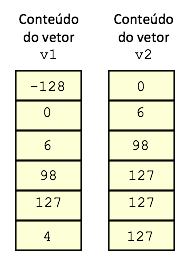
\includegraphics{"figs/image35.png"}

    \begin{figure}
\centering
\caption{image.png}
\end{figure}

    Pseudocódigo

\begin{verbatim}
método escrevaVetor(inteiro v[], inteiro n):
    para cada índice i, de i=0; até i<n; passo i=i+1 faça
        escreva(" " + v[i]);

método leiaVetor(inteiro n): retorna vetor de inteiro v[]
    vetor v de inteiros com n elementos
    para cada índice i, de i=0; até i<n; passo i=i+1 faça
        v[i] = leia("Entre com o elemento " + i + ":");
    retorne v

// Inicializações
inteiro max=0
// ENTRADA
inteiro n = leia("Digite o tamanho do vetor:");
vetores v1 e v2 de inteiros com n elementos

inteiro v1[] = leiaVetor(n)

// PROCESSAMENTO
para cada índice i, de i=0; até i<n; passo i=i+1 faça
    max = v[i]
    se i-1 >= 0 e max < v1[i-1] faça
        max = v1[i-1]
    se i+1 < n e max < v1[i+1] faça
        max = v1[i+1]
    v2[i] = max

// SAÍDA
escrevaVetor(v2)
\end{verbatim}

    \hypertarget{casos-para-teste-moodlevpl}{%
\paragraph{Casos para Teste
Moodle+VPL}\label{casos-para-teste-moodlevpl}}

Para o professor criar uma atividade VPL no Moodle para este Exemplo 04,
basta incluir em \texttt{Casos\ para\ teste}, o seguinte texto (pode
incluir mais casos):

\begin{verbatim}
case=caso1
input=6
-128
0
6
98
127
4
output=v2:
0
6
98
127
127
127
\end{verbatim}

    \begin{tcolorbox}[breakable, size=fbox, boxrule=1pt, pad at break*=1mm,colback=cellbackground, colframe=cellborder]
\prompt{In}{incolor}{ }{\boxspacing}
\begin{Verbatim}[commandchars=\\\{\}]
\PY{o}{\PYZpc{}\PYZpc{}writefile} cap5ex04.c
\PY{c+c1}{\PYZsh{}include \PYZlt{}stdio.h\PYZgt{}}
\PY{c+c1}{\PYZsh{}include \PYZlt{}stdlib.h\PYZgt{}  // malloc e free}

\PY{n+nb}{int} \PY{o}{*} \PY{n}{leiaVetor}\PY{p}{(}\PY{n+nb}{int} \PY{n}{n}\PY{p}{)} \PY{p}{\PYZob{}}
  \PY{n+nb}{int} \PY{o}{*}\PY{n}{v} \PY{o}{=} \PY{n}{malloc}\PY{p}{(}\PY{n}{n}\PY{o}{*}\PY{n}{sizeof}\PY{p}{(}\PY{n+nb}{int}\PY{p}{)}\PY{p}{)}\PY{p}{;} 
  \PY{k}{for} \PY{p}{(}\PY{n+nb}{int} \PY{n}{i} \PY{o}{=} \PY{l+m+mi}{0}\PY{p}{;} \PY{n}{i} \PY{o}{\PYZlt{}} \PY{n}{n}\PY{p}{;} \PY{n}{i}\PY{o}{+}\PY{o}{+}\PY{p}{)} \PY{p}{\PYZob{}}
    \PY{n}{scanf}\PY{p}{(}\PY{l+s+s2}{\PYZdq{}}\PY{l+s+si}{\PYZpc{}d}\PY{l+s+s2}{\PYZdq{}}\PY{p}{,} \PY{o}{\PYZam{}}\PY{n}{v}\PY{p}{[}\PY{n}{i}\PY{p}{]}\PY{p}{)}\PY{p}{;} 
  \PY{p}{\PYZcb{}}
  \PY{k}{return} \PY{n}{v}\PY{p}{;}
\PY{p}{\PYZcb{}}
\PY{n}{void} \PY{n}{escrevaVetor}\PY{p}{(}\PY{n+nb}{int} \PY{o}{*}\PY{n}{v}\PY{p}{,} \PY{n+nb}{int} \PY{n}{n}\PY{p}{)} \PY{p}{\PYZob{}}
  \PY{k}{for} \PY{p}{(}\PY{n+nb}{int} \PY{n}{i} \PY{o}{=} \PY{l+m+mi}{0}\PY{p}{;} \PY{n}{i} \PY{o}{\PYZlt{}} \PY{n}{n}\PY{p}{;} \PY{n}{i}\PY{o}{+}\PY{o}{+}\PY{p}{)} \PY{p}{\PYZob{}}
    \PY{n}{printf}\PY{p}{(}\PY{l+s+s2}{\PYZdq{}}\PY{l+s+si}{\PYZpc{}d}\PY{l+s+se}{\PYZbs{}n}\PY{l+s+s2}{\PYZdq{}}\PY{p}{,} \PY{n}{v}\PY{p}{[}\PY{n}{i}\PY{p}{]}\PY{p}{)}\PY{p}{;} 
  \PY{p}{\PYZcb{}}
\PY{p}{\PYZcb{}}
\PY{n+nb}{int} \PY{n}{main}\PY{p}{(}\PY{n}{void}\PY{p}{)} \PY{p}{\PYZob{}}
  \PY{o}{/}\PY{o}{/} \PY{n}{ENTRADA} \PY{n}{DE} \PY{n}{DADOS}
  \PY{n+nb}{int} \PY{n}{n}\PY{p}{,} \PY{o}{*}\PY{n}{v1}\PY{p}{;}   \PY{o}{/}\PY{o}{/} \PY{n}{variaveis} \PY{n}{de} \PY{n}{referência} \PY{n}{v1}
  \PY{n}{printf}\PY{p}{(}\PY{l+s+s2}{\PYZdq{}}\PY{l+s+s2}{Digite o tamanho do vetor: }\PY{l+s+s2}{\PYZdq{}}\PY{p}{)}\PY{p}{;}
  \PY{n}{scanf}\PY{p}{(}\PY{l+s+s2}{\PYZdq{}}\PY{l+s+si}{\PYZpc{}d}\PY{l+s+s2}{\PYZdq{}}\PY{p}{,} \PY{o}{\PYZam{}}\PY{n}{n}\PY{p}{)}\PY{p}{;}
  \PY{n+nb}{int} \PY{o}{*}\PY{n}{v2} \PY{o}{=} \PY{n}{malloc}\PY{p}{(}\PY{l+m+mi}{100}\PY{o}{*}\PY{n}{sizeof}\PY{p}{(}\PY{n+nb}{int}\PY{p}{)}\PY{p}{)}\PY{p}{;}
  \PY{n}{printf}\PY{p}{(}\PY{l+s+s2}{\PYZdq{}}\PY{l+s+s2}{Digite os elementos: }\PY{l+s+s2}{\PYZdq{}}\PY{p}{)}\PY{p}{;}
  \PY{n}{v1} \PY{o}{=} \PY{n}{leiaVetor}\PY{p}{(}\PY{n}{n}\PY{p}{)}\PY{p}{;}
  \PY{o}{/}\PY{o}{/} \PY{n}{PROCESSAMENTO}
  \PY{k}{for} \PY{p}{(}\PY{n+nb}{int} \PY{n}{i} \PY{o}{=} \PY{l+m+mi}{0}\PY{p}{;} \PY{n}{i} \PY{o}{\PYZlt{}} \PY{n}{n}\PY{p}{;} \PY{n}{i}\PY{o}{+}\PY{o}{+}\PY{p}{)} \PY{p}{\PYZob{}}
    \PY{n+nb}{int} \PY{n+nb}{max} \PY{o}{=} \PY{n}{v1}\PY{p}{[}\PY{n}{i}\PY{p}{]}\PY{p}{;}
    \PY{k}{if} \PY{p}{(}\PY{n}{i}\PY{o}{\PYZhy{}}\PY{l+m+mi}{1} \PY{o}{\PYZgt{}}\PY{o}{=} \PY{l+m+mi}{0} \PY{o}{\PYZam{}}\PY{o}{\PYZam{}} \PY{n+nb}{max} \PY{o}{\PYZlt{}} \PY{n}{v1}\PY{p}{[}\PY{n}{i}\PY{o}{\PYZhy{}}\PY{l+m+mi}{1}\PY{p}{]}\PY{p}{)}
        \PY{n+nb}{max} \PY{o}{=} \PY{n}{v1}\PY{p}{[}\PY{n}{i}\PY{o}{\PYZhy{}}\PY{l+m+mi}{1}\PY{p}{]}\PY{p}{;}
    \PY{k}{if} \PY{p}{(}\PY{n}{i}\PY{o}{+}\PY{l+m+mi}{1} \PY{o}{\PYZlt{}} \PY{n}{n} \PY{o}{\PYZam{}}\PY{o}{\PYZam{}} \PY{n+nb}{max} \PY{o}{\PYZlt{}} \PY{n}{v1}\PY{p}{[}\PY{n}{i}\PY{o}{+}\PY{l+m+mi}{1}\PY{p}{]}\PY{p}{)}
        \PY{n+nb}{max} \PY{o}{=} \PY{n}{v1}\PY{p}{[}\PY{n}{i}\PY{o}{+}\PY{l+m+mi}{1}\PY{p}{]}\PY{p}{;}
    \PY{n}{v2}\PY{p}{[}\PY{n}{i}\PY{p}{]} \PY{o}{=} \PY{n+nb}{max}\PY{p}{;}
  \PY{p}{\PYZcb{}}
  \PY{o}{/}\PY{o}{/} \PY{n}{SAÍDA}\PY{p}{:}
  \PY{n}{printf}\PY{p}{(}\PY{l+s+s2}{\PYZdq{}}\PY{l+s+se}{\PYZbs{}n}\PY{l+s+s2}{v2:}\PY{l+s+se}{\PYZbs{}n}\PY{l+s+s2}{\PYZdq{}}\PY{p}{)}\PY{p}{;}
  \PY{n}{escrevaVetor}\PY{p}{(}\PY{n}{v2}\PY{p}{,}\PY{n}{n}\PY{p}{)}\PY{p}{;}
  \PY{n}{free}\PY{p}{(}\PY{n}{v1}\PY{p}{)}\PY{p}{;} \PY{o}{/}\PY{o}{/} \PY{n}{liberar} \PY{n}{memória} \PY{n}{alocado} \PY{n}{com} \PY{n}{malloc}
  \PY{n}{free}\PY{p}{(}\PY{n}{v2}\PY{p}{)}\PY{p}{;}
  \PY{k}{return} \PY{l+m+mi}{0}\PY{p}{;}
\PY{p}{\PYZcb{}}
\end{Verbatim}
\end{tcolorbox}

    \begin{tcolorbox}[breakable, size=fbox, boxrule=1pt, pad at break*=1mm,colback=cellbackground, colframe=cellborder]
\prompt{In}{incolor}{ }{\boxspacing}
\begin{Verbatim}[commandchars=\\\{\}]
\PY{o}{\PYZpc{}\PYZpc{}}\PY{k}{shell}
gcc cap5ex04.c \PYZhy{}o output2
./output2
\end{Verbatim}
\end{tcolorbox}

    \hypertarget{exercuxedcios}{%
\subsection{Exercícios}\label{exercuxedcios}}

    Ver notebook Colab nos arquivos \texttt{cap5.partX.lab.*.ipynb}
(\texttt{X} \(\in\) \texttt{{[}2,3{]}} e \texttt{*} é a extensão da
linguagem), utilizando alguma linguagem de programação de sua
preferência, organizadas em subpastas contidas de \texttt{"gen"}, na
pasta do Google Drive
\href{https://drive.google.com/drive/folders/1YlFwv8XYN7PYYf-HwDMlkxzbmXzJw9cM?usp=sharing}{colabs}.

    \hypertarget{atividades-no-moodlevpl}{%
\subsection{Atividades no Moodle+VPL}\label{atividades-no-moodlevpl}}

Algumas atividades no Moodle+VPL pedem como entradas vetores de inteiros
(ou reais), \textbf{armazenados em uma única linha}. Exemplo de entrada
a ser lida:

\hypertarget{entrada-de-dados-cada-linha-contem-um-texto-ou-string-incluindo-os-elementos-do-vetor-e-vuxe1rios-espauxe7os}{%
\subsubsection{\texorpdfstring{Entrada de Dados (cada linha contem um
texto ou \emph{string} incluindo os elementos do vetor e vários espaços
``\texttt{}''):}{Entrada de Dados (cada linha contem um texto ou string incluindo os elementos do vetor e vários espaços ``\,''):}}\label{entrada-de-dados-cada-linha-contem-um-texto-ou-string-incluindo-os-elementos-do-vetor-e-vuxe1rios-espauxe7os}}

\begin{verbatim}
7 3 7 9 7 7 0 9 8 4 8 9 0 1 7 8 4 1 1 0 
2 1 9 4 3 6 0 9 8 4 2 8 0 6 7 3 2 4 5 9
\end{verbatim}

Para não ter que incluir várias entradas inteiras, a melhor solução é
fazer um método de leitura, passando como argumento um texto
(\emph{string}) referente a cada linha. Esse método deve retornar o
vetor.

    \begin{tcolorbox}[breakable, size=fbox, boxrule=1pt, pad at break*=1mm,colback=cellbackground, colframe=cellborder]
\prompt{In}{incolor}{123}{\boxspacing}
\begin{Verbatim}[commandchars=\\\{\}]
\PY{o}{\PYZpc{}\PYZpc{}writefile} str2int.c
\PY{c+c1}{\PYZsh{}include \PYZlt{}stdio.h\PYZgt{}}
\PY{c+c1}{\PYZsh{}include \PYZlt{}string.h\PYZgt{}}
\PY{c+c1}{\PYZsh{}include \PYZlt{}stdlib.h\PYZgt{}}

\PY{n+nb}{int} \PY{n}{main}\PY{p}{(}\PY{p}{)} \PY{p}{\PYZob{}}
   \PY{n}{char} \PY{n}{string}\PY{p}{[}\PY{p}{]} \PY{o}{=} \PY{l+s+s2}{\PYZdq{}}\PY{l+s+s2}{7 3 7 9 7 7 0 9 8 4 8 9 0 1     7 8 4 1 1 0     }\PY{l+s+s2}{\PYZdq{}}\PY{p}{;}
   \PY{n}{char} \PY{o}{*} \PY{n}{token} \PY{o}{=} \PY{n}{strtok}\PY{p}{(}\PY{n}{string}\PY{p}{,} \PY{l+s+s2}{\PYZdq{}}\PY{l+s+s2}{ }\PY{l+s+s2}{\PYZdq{}}\PY{p}{)}\PY{p}{;}
   \PY{n+nb}{int} \PY{n}{v}\PY{p}{[}\PY{l+m+mi}{100}\PY{p}{]}\PY{p}{;}
   \PY{n+nb}{int} \PY{n}{i} \PY{o}{=} \PY{l+m+mi}{0}\PY{p}{;}
   \PY{k}{while}\PY{p}{(} \PY{n}{token} \PY{o}{!=} \PY{n}{NULL} \PY{p}{)} \PY{p}{\PYZob{}}
      \PY{n}{v}\PY{p}{[}\PY{n}{i}\PY{o}{+}\PY{o}{+}\PY{p}{]} \PY{o}{=} \PY{n}{atoi}\PY{p}{(}\PY{n}{token}\PY{p}{)}\PY{p}{;} \PY{o}{/}\PY{o}{/} \PY{n}{converte} \PY{n}{texto} \PY{n}{para} \PY{n}{inteiro}
      \PY{n}{token} \PY{o}{=} \PY{n}{strtok}\PY{p}{(}\PY{n}{NULL}\PY{p}{,} \PY{l+s+s2}{\PYZdq{}}\PY{l+s+s2}{ }\PY{l+s+s2}{\PYZdq{}}\PY{p}{)}\PY{p}{;}
   \PY{p}{\PYZcb{}}
   \PY{n+nb}{int} \PY{n}{n}\PY{o}{=}\PY{n}{i}\PY{p}{;}
   \PY{k}{for} \PY{p}{(}\PY{n}{i}\PY{o}{=}\PY{l+m+mi}{0}\PY{p}{;}\PY{n}{i}\PY{o}{\PYZlt{}}\PY{n}{n}\PY{p}{;}\PY{n}{i}\PY{o}{+}\PY{o}{+} \PY{p}{)}\PY{p}{\PYZob{}}
     \PY{n}{printf}\PY{p}{(}\PY{l+s+s2}{\PYZdq{}}\PY{l+s+si}{\PYZpc{}d}\PY{l+s+s2}{ }\PY{l+s+s2}{\PYZdq{}}\PY{p}{,}\PY{n}{v}\PY{p}{[}\PY{n}{i}\PY{p}{]}\PY{p}{)}\PY{p}{;}
   \PY{p}{\PYZcb{}}
   \PY{k}{return} \PY{l+m+mi}{0}\PY{p}{;}
\PY{p}{\PYZcb{}}
\end{Verbatim}
\end{tcolorbox}

    \begin{tcolorbox}[breakable, size=fbox, boxrule=1pt, pad at break*=1mm,colback=cellbackground, colframe=cellborder]
\prompt{In}{incolor}{124}{\boxspacing}
\begin{Verbatim}[commandchars=\\\{\}]
\PY{o}{\PYZpc{}\PYZpc{}}\PY{k}{shell}
gcc str2int.c \PYZhy{}o output2
./output2
\end{Verbatim}
\end{tcolorbox}

    \hypertarget{entrada-de-dados-a-linha-contem-um-texto-ou-string}{%
\subsubsection{\texorpdfstring{Entrada de Dados (a linha contem um texto
ou
\emph{string}):}{Entrada de Dados (a linha contem um texto ou string):}}\label{entrada-de-dados-a-linha-contem-um-texto-ou-string}}

\begin{verbatim}
A UFABC completou 15 anos!
\end{verbatim}

Como contar as vogais de um texto?

    \hypertarget{revisuxe3o-deste-capuxedtulo-de-vetores}{%
\subsection{Revisão deste capítulo de
Vetores}\label{revisuxe3o-deste-capuxedtulo-de-vetores}}

\begin{itemize}
\tightlist
\item
  Introdução \textgreater{} Vetores são estruturas para armazenar vários
  elementos de um mesmo tipo de dados em uma única variável.
\item
  Trabalhando com vetores \textgreater{} Cada linguagem possui uma
  sintaxe própria para declarar e alocar vetores.
\item
  Acessando elementos de um vetor \textgreater{} ATENÇÃO para não
  acessar uma posição do vetor não reservada/alocada, geralmente
  \texttt{\textless{}0} e \texttt{\textgreater{}=n}.
\item
  Formas de percorrer um vetor \textgreater{} É possível varrer um vetor
  na forma \textbf{\emph{raster}} e \textbf{\emph{anti-raster}}, também
  usando diferentes passos, mas geralmente é passo=1.
\item
  Modularização e vetores \textgreater{} Muito útil usar principalmente
  os módulos de \texttt{leiaVetor} e \texttt{escrevaVetor}, podendo ser
  reaproveitados em vários códigos.
\item
  Exercícios
\item
  Revisão deste capítulo de Vetores
\end{itemize}


    % Add a bibliography block to the postdoc
    
    
    
\end{document}
